\chapter{Empirical Attribution of Failure Modes}
\label{ch:empirical}

This chapter is adapted from \textbf{Locating Failure in Multi-Page Visually Rich Document Understanding: An Empirical Attribution}~\cite{xu2026locating}, by \textbf{Lewei Xu}, Yihao Ding, Zihan Xu, Daniel Yitian Su, Daochang Liu, Siwen Luo, Yifan Peng, and Wei Liu, \emph{submitted to EACL and currently under review}. The first author was responsible for formulating the failure taxonomy and attribution framework; designing the experimental methodology; implementing and running all experiments; analysing and interpreting the results; and preparing the full manuscript, including the main text, methodological details, empirical analysis, figures and tables, and appendix material. 

\section{Introduction}
Multi-page visually rich document understanding has advanced rapidly, but it remains difficult to determine why these systems fail. Modern MP-VRDU pipelines combine document encoding, evidence selection, and multimodal reasoning, and errors at any one stage can propagate to the final answer. As a result, improvements to one component are often evaluated only through end-to-end accuracy, making it difficult to distinguish whether a gain comes from better representation, better evidence selection, or better use of the evidence already available. This makes failure attribution an important complement to the system-level organisation developed in the previous chapter.

The literature reflects substantial disagreement about what limits MP-VRDU systems. OCR-free methods argue that operating directly on page images avoids information loss introduced by text extraction and preserves visual and layout cues that may be difficult to recover from parsed text \citep{tanaka2025vdocrag, zheng2026doc, cho2024m3docrag}. Other studies instead find that vision-only reasoners remain weaker on dense textual content and that combining textual and visual representations can outperform either alone \citep{hannan2026docslm, han2025mdocagent, suri2025visdom}, while some report the opposite, with vision-only pipelines outperforming combined representations \citep{liu2025resolving}. Retrieval findings are similarly mixed. Retrieving too little evidence can omit information needed to answer the question \citep{yan2026docseeker, li2026avir}, whereas retrieving too much can introduce irrelevant context, attention dilution, and position-dependent degradation \citep{liu2024lost, wang2024needle, pez2025enhancing}. Some work therefore prioritises broad evidence coverage \citep{liu2025resolving, zhu2026doclens}, while others emphasise reranking or adaptive retrieval to reduce irrelevant context \citep{li2026avir, pez2025enhancing}. Reasoning failures have likewise been attributed to difficulty combining evidence across pages \citep{zheng2026doc}, errors in interpreting evidence within individual pages \citep{guo2026end}, and a tendency to answer even when the available evidence is insufficient \citep{landeghem2023document, zhang2025dream, ma2024mmlongbench}. We interpret these competing claims as evidence of three distinct loci at which MP-VRDU systems can fail: \textbf{representation, selection, and reasoning}.

\textbf{Our contributions are as follows:} \textbf{(1)} We introduce an attribution framework that formalises MP-VRDU failure through three system-level loci: representation, selection, and reasoning (\S\ref{sec:attribution_framework}). \textbf{(2)} We conduct a controlled empirical study that intervenes on one locus at a time to isolate the mechanisms underlying each and test competing claims about modality, evidence selection, and reasoning under a unified experimental setting (\S\ref{sec:emp_methodology}, \S\ref{sec:emp_findings}). \textbf{(3)} We analyse the resulting error patterns and derive practical implications for the design and deployment of MP-VRDU systems under constrained compute budgets (\S\ref{sec:emp_error_analysis}, \S\ref{sec:practical_discussion}).

\section{Related Work}
\label{sec:relatedwork}
% Most evaluations of representations, retrievers, and reasoners report end-to-end accuracy, which registers that a method improved a system without identifying the stage responsible \citep{tanaka2025vdocrag, han2025mdocagent, suri2025visdom, yan2026docseeker}. 
OCR-cascade studies isolate the encoding stage and trace a parser mistake as it propagates untouched through a text-only pipeline, in which no image channel is present to recover the corrupted content \citep{zhang2025ocr}. Component ablations isolate the selection stage instead, finding that most gain comes from running a short retrieval loop rather than from adapting it \citep{shaikh2026dissecting} and that the retrieval algorithm matters more than the generator \citep{ke2026not}, though both operate over pre-segmented text corpora in which no encoding stage enters the accounting. Faithfulness diagnostics trace how evidence is used after retrieval, and both facet-level tracing \citep{elchafei2026facet} and Graph-RAG decompositions \citep{zarrinkia2026reasoning} find the gold answer present in most retrieved contexts and attribute the residual error to integration rather than retrieval, on text and without the cross-page structure that makes integration hard. Unified benchmarks improve comparability by scoring retrieval paradigms for visually rich documents under one protocol \citep{peng2025unidoc}, yet compare whole pipelines, so a difference is attributable to a paradigm rather than to a stage within it. Each of these studies isolates one stage with the others held absent, or aggregates over all of them. None intervenes stage by stage within a single multi-page pipeline, which is what attributes an error to the encoding, the selection, or the reasoning, and places the field's competing claims at the locus each concerns.

\section{Attribution Framework}
\label{sec:attribution_framework}

\begin{figure*}[h]
\centering
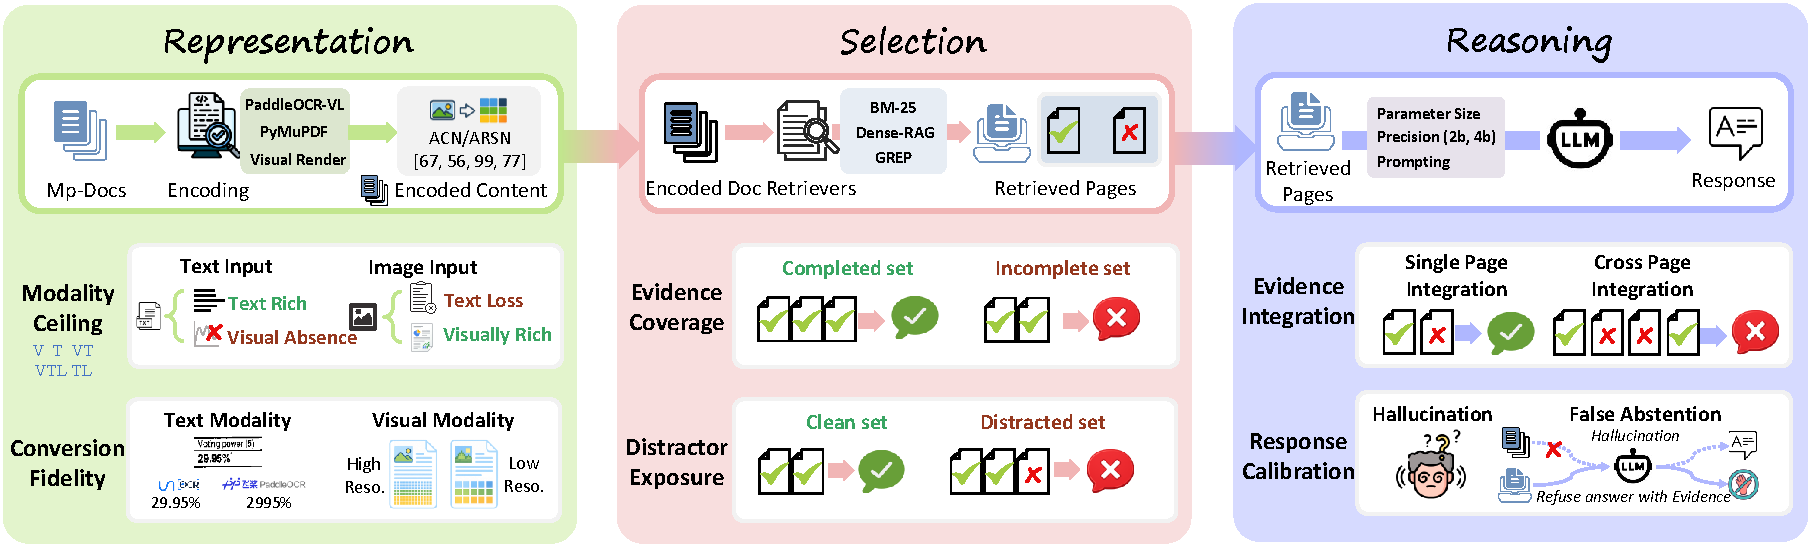
\includegraphics[width=\linewidth]{empirical/framework.pdf}
\caption{The three failure modes and their mechanisms.}
\label{fig:framework}
\end{figure*}

An incorrect answer arises at one of three failure loci. \textbf{Representation} fails when the encoding does not preserve the evidence a question needs. \textbf{Selection} fails when the required evidence is missing from, or diluted within, what reaches the reasoner. \textbf{Reasoning} fails when the reasoner cannot combine the evidence it holds, or misjudges whether that evidence supports an answer. The three are hierarchical: evidence lost in encoding cannot be selected, and evidence never selected cannot be reasoned over. This allows attribution to be possible, since a locus can be tested only once those above it are neutralised.

Because the loci are defined by system function rather than architecture, the techniques surveyed in Chapter~\ref{ch:survey} reduce failure at one or more of them rather than forming categories of their own. Some act on a single locus. Retrieval and reranking change what evidence reaches the reasoner without altering how the document is encoded or how the reasoner integrates it. Others act on several at once. An agentic controller mainly addresses selection, gathering evidence over several rounds rather than in one fixed pass, but can also act on representation when it re-renders a region at higher resolution, and on reasoning when it revises an answer through self-refinement.

\subsection{Representation}
\label{sec:fm_representation}
Representation is the conversion of the document into an artifact the later stages consume. That artifact may be the embedded text layer, parser markdown, a cropped page region, the rendered page image, or a combination of these. What happens after the artifact is tokenised, such as projection, resampling, or compression, belongs to the reasoning locus, since it is a property of the backbone rather than of the conversion. The choice of artifact therefore fixes both what a document can express and the cost of conversion. Representation failures occur through two mechanisms:
\paragraph{(1) Modality Ceiling.} Each modality can represent only a bounded range of signals. A representation preserves a signal only when its modality can encode it and at the granularity permitted by its representation. For example, text tokens cannot capture non-linguistic information, and visual tokens express fine-grained details only when sufficient spatial resolution and token budget are available.
\paragraph{(2) Conversion Fidelity.} For signals that a modality can represent, conversion fidelity measures how accurately the encoding reproduces them. Failures occur when the conversion degrades or corrupts a signal that the modality could otherwise carry. For instance, a document parser may misread a numeric value and cause the downstream reasoner to operate on an incorrect but seemingly reliable representation \citep{zhang2025ocr}.

\subsection{Selection}
\label{sec:fm_selection}
Selection decides which parts of the encoded document are placed before the reasoner. The operation exists only in the multi-page setting, where the whole document does not fit in context. Similarity retrieval is a common instantiation but not the only one: techniques such as structural navigation, adaptive re-ranking and agentic inspection all deliver evidence often across many iterations (\S\ref{sec:tf-retrieval}, \S\ref{sec:tf-agentic}). Granularity is a further choice; most systems select whole pages, matching benchmark annotations and late-interaction retrievers, though a section, a table, or a cropped figure can serve as the unit. 
% Coarser units carry surrounding material along with the evidence, while finer ones raise precision at the risk of cutting through an evidence unit. 
Selection failures arise through two mechanisms:
\paragraph{(1) Evidence Coverage.} This mechanism measures how much of the evidence required to answer a question is present in the selected context, \emph{i.e.}, the recall of the required evidence units. Omitting required evidence leaves the reasoner with an incomplete evidence set, placing an upper bound on downstream accuracy regardless of the reasoner's capability.
\paragraph{(2) Distractor Exposure.} Selection may also deliver evidence that is irrelevant to the question. This mechanism measures the extent to which distractors accompany the required evidence. Unlike omission, distractors do not by themselves make the evidence insufficient, but they increase the burden on the reasoner to identify and use the relevant content.

\subsection{Reasoning}
\label{sec:fm_reasoning}
Reasoning produces an answer from the evidence the earlier two stages deliver. This locus is what remains once the representation carries the evidence a question needs and the selection places that evidence before the reasoner. 
% Even then, failure may arise from ambiguous or underspecified questions, which belong to no locus, being a property of the data itself. 
If the evidence is provided to the reasoner at sufficient fidelity and completeness, the remaining failures can only be attributed to the reasoner itself. Repair can come in the form of instruction, scale, architecture, or training (\S\ref{sec:tf-reasoning}, \S\ref{sec:train-reasoning}). Unlike representation and selection, reasoning failures can arise through many mechanisms, such as arithmetic error over correctly read values or answering a different question from the one asked; we focus on two multi-page specific failures:
\paragraph{(1) Evidence Integration.} Multi-page questions may require the reasoner to combine complementary information from several pages, including content whose meaning spans page boundaries. A model may succeed when all relevant evidence is given but fail when it must connect distributed evidence on its own. This difficulty may be amplified in long contexts, where evidence at different positions is not used equally reliably \citep{liu2024lost}.
\paragraph{(2) Response Calibration.} This mechanism concerns whether the model aligns its response with the level of support provided by the available evidence. Unlike integration, calibration is tested both when sufficient evidence is present and when it is absent by construction. Failures occur in two directions: \emph{hallucination}, where the model produces an answer unsupported by the available evidence \citep{li2023survey}, and \emph{false abstention}, where it refuses to answer despite having sufficient evidence. We treat these as a single mechanism because they represent opposite sides of the same decision, so an intervention that reduces one tends to increase the other \citep{whitehead2022reliable}.

\section{Methodology}
\label{sec:emp_methodology}
We instantiate the framework in a \textbf{single-pass retriever--generator} document question answering system, evaluated over two MP-VRDU benchmarks whose annotations make the controlled experiments possible. We first describe the system and the attribution experiments that isolate each mechanism (\S\ref{sec:attribution}), followed by the experimental configurations of representation, selection, and reasoning (\S\ref{sec:emp_representation}--\S\ref{sec:emp_reasoning}), including additional experiments comparing practical pipeline choices (\S\ref{sec:emp_additional}). We then describe the two datasets (\S\ref{sec:emp_mmlongbench}, \S\ref{sec:emp_longdocurl}) and conclude with the evaluation protocol (\S\ref{sec:emp_evaluation}).
\subsection{Attribution by Construction}
\label{sec:attribution}

The document question answering system consists of three stages that correspond to the three failure loci described in \S\ref{sec:attribution_framework}. For each question, the system performs the following:

\begin{enumerate}
    \item \textbf{Encoding Stage:} every page of the document is converted into the representation the later stages consume, as parser markdown, a rendered page image, or both. The conversion runs once per document and is cached, so the same encoded pages serve every question over that document and no question changes what a page contains.
    \item \textbf{Retrieval Stage:} a retriever scores every encoded page against the question and returns the highest-ranked $k$. Scoring is at page granularity, matching the annotation granularity of both datasets, so a retrieved unit and an annotated evidence unit are the same object. The selected pages are restored to document order before assembly, so a page's position in the context reflects the document rather than its rank.
    \item \textbf{Inference Stage:} a multimodal LLM receives the assembled pages, the question, and an instruction describing the task, and emits an answer in a single pass. It sees nothing else of the document, and no output is fed back to an earlier stage.
\end{enumerate}

The system's stages act once and in order, allowing failures to be attributed by constructing conditions that isolate one locus while holding the others fixed. Across the six mechanisms defined in \S\ref{sec:attribution_framework}, we vary the relevant representation, evidence, or reasoning condition and compare relevant metrics against an appropriate controlled baseline. Table~\ref{tab:experiments} summarises these experiments.

The default configuration is fixed across the study: pages are encoded at \textbf{TLV}, retrieved by ColQwen3, and fed to Qwen3-VL-8B-Instruct in \texttt{bf16} with greedy decoding and no instruction beyond the question. Each mechanism experiment changes only the condition required to test that failure while keeping other stages fixed.
% Additional configuration and intervention experiments likewise replace individual components within this controlled pipeline, allowing their effects to be distinguished from changes elsewhere in the system.

\begin{table}[h]
\centering
\small
\setlength{\tabcolsep}{4pt}
\renewcommand{\arraystretch}{1.15}
\begin{tabularx}{\linewidth}{@{}
  >{\raggedright\arraybackslash}p{2.3cm}
  l
  >{\raggedright\arraybackslash}X
  >{\raggedright\arraybackslash}X@{}}
\toprule
Locus & Mechanism & Constructed condition & Held fixed \\
\midrule
\multirow{3}{2.3cm}{\textbf{Representation}\\(Encoding stage: \S\ref{sec:emp_representation})}
 & Modality ceiling & Encoding rung compared across T, TL, TLV, V by evidence source & Gold pages, reasoner, prompt \\
\cmidrule(l){2-4}
 & Conversion fidelity & Text and image fidelity across three parsers and three render resolutions & Encoding rung, gold pages, reasoner, prompt \\
\midrule
\multirow{3}{2.3cm}{\textbf{Selection}\\(Retrieval stage: \S\ref{sec:emp_selection})}
 & Evidence coverage & Gold pages withheld from multi-page questions & Encoding, reasoner, prompt \\
\cmidrule(l){2-4}
 & Distractor exposure & Non-gold pages added at a fixed gold-page count & Gold set, encoding, reasoner, prompt \\
\midrule
\multirow{3}{2.3cm}{\textbf{Reasoning}\\(Inference stage: \S\ref{sec:emp_reasoning})}
 & Evidence integration & Evidence conditions requiring cross-page integration & Documents, gold pages, encoding \\
\cmidrule(l){2-4}
 & Response calibration & Answerable and unsupported evidence conditions & Gold pages, encoding, reasoner \\
\bottomrule
\end{tabularx}
\caption{Attribution by construction: conditions used to isolate failures.}
\label{tab:experiments}
\end{table}

\subsection{Representation Experiments}
\label{sec:emp_representation}

Each page is encoded from two signals: a text channel and the page image. The representation experiments run only on questions answerable from their annotated evidence, and modality comparisons are analysed according to the source from which that evidence must be recovered.

\begin{table}[h]
\centering
\small
\setlength{\tabcolsep}{4pt}
\renewcommand{\arraystretch}{1.15}
\begin{tabularx}{\linewidth}{@{}
  >{\raggedright\arraybackslash}p{1.1cm}
  >{\raggedright\arraybackslash}p{2.9cm}
  >{\raggedright\arraybackslash}p{1.8cm}
  >{\raggedright\arraybackslash}p{2.4cm}
  >{\raggedright\arraybackslash}X@{}}
\toprule
Rung & Text channel & Image & Cost & Role \\
\midrule
T & Embedded text (PyMuPDF) & -- & Extraction only & Acquisition floor; empty on scanned pages \\
\midrule
TL & Parser markdown & -- & Parser pass & Text-only ceiling; recovers reading order and table structure \\
\midrule
TLV & Parser markdown & Page image & Parser pass + vision tokens & Combined encoding; the only full option on scanned pages \\
\midrule
V & -- & Page image & Vision tokens & Vision-only \\
\bottomrule
\end{tabularx}
\caption{Representation ladder. Ordered by fidelity and, as a consequence, by cost.}
\label{tab:ladder_def}
\end{table}


\paragraph{Modality ceiling.} We vary which signals reach the reasoner at all, across the four rungs of Table~\ref{tab:ladder_def}: embedded text (\textbf{T}), layout-aware parser text (\textbf{TL}), parser text combined with the page image (\textbf{TLV}), and the page image alone (\textbf{V}). The comparison tests whether the required evidence remains recoverable when textual, structural, or visual signals are unavailable, rather than assuming that one representation is uniformly preferable across question types.

\begin{table}[h]
\centering
\small
\setlength{\tabcolsep}{5pt}
\renewcommand{\arraystretch}{1.15}
\begin{tabular}{@{}lrl@{\hskip 1.2em\vrule\hskip 1.2em}lrrl@{}}
\toprule
\multicolumn{3}{@{}l}{\textit{Parser} (text channel)} & \multicolumn{4}{l@{}}{\textit{Resolution} (image channel)} \\
\cmidrule(r){1-3} \cmidrule(l){4-7}
Parser & Params & Rungs & Preset & Tokens & Pixel cap & Rungs \\
\cmidrule(r){1-3} \cmidrule(l){4-7}
PaddleOCR-VL & 0.9B & TL, TLV & low & 400 & 313,600 & TLV, V \\
\cmidrule(r){1-3} \cmidrule(l){4-7}
MinerU 2.5 & 1.2B & TL, TLV & med & 640 & 501,760 & TLV, V \\
\cmidrule(r){1-3} \cmidrule(l){4-7}
Unlimited-OCR & 3.3B & TL, TLV & high & 960 & 752,640 & TLV, V \\
\bottomrule
\end{tabular}
\caption{Representation fidelity variation. PaddleOCR-VL and \texttt{med} are the defaults; the two halves vary independently.}
\label{tab:fidelity}
\end{table}

\paragraph{Conversion fidelity.} We vary the quality of each channel while holding the representation rung fixed, through the parser for text and the render resolution for the image (Table~\ref{tab:fidelity}). These experiments test whether information that a modality can in principle represent is degraded before reaching the reasoner, and whether improving the fidelity of that conversion improves downstream performance.

\paragraph{Configuration.} The \textbf{T} rung supplies the PDF's embedded text layer, read directly with PyMuPDF, while \textbf{TL} supplies markdown produced by a layout-aware parser that applies OCR where required. \textbf{TLV} combines this parser markdown with the rendered page image, and \textbf{V} supplies the image alone; no bounding boxes or other explicit layout signals are passed to the reasoner. The default parser is PaddleOCR-VL (0.9B)~\citep{cui2025paddleocr}, run through the \texttt{paddleocr} 3.7 pipeline with PP-DocLayoutV2 layout analysis, PP-OCRv5 detection and recognition, and orientation and unwarping enabled. MinerU 2.5 (1.2B)~\citep{niu2026mineru2} and Unlimited-OCR (3.3B)~\citep{yin2026unlimited} provide the parser comparisons. Pages are rasterised at 200 DPI and downsampled to a per-page pixel budget before inference, since the backbone packs one vision token per $28 \times 28$ patch. Every experiment uses the \texttt{med} image preset except the resolution sweep, which evaluates all three presets. A fifth encoding, \textbf{TV}, combines embedded text with the page image without parsing and is used as a direct contrast against \textbf{TLV}.

\subsection{Selection Experiments}
\label{sec:emp_selection}
Selection determines which evidence reaches the reasoner. We investigate failures caused by incomplete evidence coverage and by exposure to irrelevant pages.

\begin{table}[h]
\centering
\small
\setlength{\tabcolsep}{5pt}
\renewcommand{\arraystretch}{1.15}
\begin{tabularx}{\linewidth}{@{}>{\raggedright\arraybackslash}p{2.5cm}>{\raggedright\arraybackslash}X>{\raggedright\arraybackslash}p{2.1cm}>{\raggedright\arraybackslash}p{2.9cm}@{}}
\toprule
Rule & Pages supplied & Blocking & Range \\
\midrule
\texttt{drop\_top} & All gold except the highest-ranked & $\geq 2$ gold & -- \\
\texttt{drop\_bottom} & All gold except the lowest-ranked & $\geq 2$ gold & -- \\
\texttt{keep\_top} & The highest-ranked gold page only & $\geq 2$ gold & -- \\
\texttt{keep\_bottom} & The lowest-ranked gold page only & $\geq 2$ gold & -- \\
\midrule
$+k$ distractors & All gold plus the $k$ top-ranked non-gold pages & Exactly 1 gold & $k \in \{1,2,3,4,5\}$ \\
$+k$ distractors & All gold plus the $k$ top-ranked non-gold pages & Exactly 2 gold & $k \in \{1,2,3,4\}$ \\
% $+k$ distractors & All gold plus the $k$ top-ranked non-gold pages & Exactly 3 gold & $k \in \{1,2,3\}$ \\
\bottomrule
\end{tabularx}
\caption{Gold set perturbations for selection experiments. Read against the oracle condition of all gold pages with no distractors. The distractor rules hold the supplied set at six pages or fewer regardless of gold count.}
\label{tab:page_set}
\end{table}

\paragraph{Evidence coverage.} We vary how much of the required evidence reaches the reasoner by withholding gold pages from questions that cite more than one. These conditions run on multi-page questions only and are evaluated against the corresponding complete gold-page oracle. Pages are ranked by ColQwen3 within the document, allowing us to remove either the highest- or lowest-ranked gold page, or retain only one of them. A condition that a question cannot satisfy is excluded and recorded rather than silently satisfied with a different page set.

\paragraph{Distractor exposure.} We vary how much irrelevant evidence accompanies the required evidence by adding top-ranked non-gold pages to a complete gold set. Conditions are blocked on the exact gold-page count, so questions requiring different amounts of evidence are not pooled at the same retrieval depth. The range of $k$ narrows as the gold count rises, keeping the supplied context at six pages or fewer and preventing distractor count from being confounded with arbitrary increases in context length.

\paragraph{Configuration.} ColQwen3 is used to rank both gold and non-gold pages for the constructed selection conditions. As a late-interaction visual retriever, it scores the question directly against each rendered page image rather than its extracted text. For evidence coverage, ranking is restricted to the annotated gold set; for distractor exposure, non-gold pages are ranked separately and the highest-scoring pages are appended to the complete gold set. The constructed page sets are evaluated across the \textbf{T}, \textbf{TL}, \textbf{TLV}, and \textbf{V} representations, with verdict transitions additionally computed against the corresponding \textbf{TLV} oracle condition.

\subsection{Reasoning Experiments}
\label{sec:emp_reasoning}

Reasoning determines how the available evidence is used to produce a response. We investigate failures in integrating evidence across the supplied context and in calibrating responses to the support that evidence provides.

% \begin{table}[h]
\centering
\small
\setlength{\tabcolsep}{4pt}
\renewcommand{\arraystretch}{1.15}
\begin{tabularx}{\linewidth}{@{}
  >{\raggedright\arraybackslash}p{2.7cm}
  >{\raggedright\arraybackslash}p{3.0cm}
  >{\raggedright\arraybackslash}X@{}}
\toprule
\textbf{Mechanism} & \textbf{Question pool} & \textbf{Experimental condition} \\
\midrule
\textbf{Evidence integration}
& Answerable questions
& Compare questions whose annotated evidence is contained on a single page with questions requiring evidence across multiple pages; all annotated evidence pages are supplied. \\
\midrule
\textbf{Response calibration}
& Answerable and unanswerable questions
& Compare responses when sufficient evidence is available with responses when the supplied context does not support an answer, measuring both unsupported answers and false abstentions. \\
\bottomrule
\end{tabularx}
\caption{Reasoning attribution experiments. Representation and selection failures are controlled by supplying the relevant evidence directly to the reasoner.}
\label{tab:reasoning_experiments}
\end{table}

\paragraph{Evidence integration.} We test evidence integration by separating questions according to the structure of the evidence required to answer them while supplying the annotated evidence directly to the reasoner. The resulting question pools distinguish evidence that can be resolved from an individual page from evidence that must be combined across multiple pages.

\begin{table}[h]
\centering
\small
\begin{tabular}{lp{0.68\textwidth}}
\toprule
Mode & Instruction \\
\midrule
\texttt{none} & (empty) \\
\texttt{grounded} & Use only the provided document evidence and keep the answer concise. \\
\texttt{abstain} & \texttt{grounded}, plus: If the evidence does not contain the answer, answer exactly: Not answerable. \\
\texttt{abstain\_balanced} & \texttt{abstain}, plus: If the evidence does contain the answer, give it: do not decline a question the evidence supports. \\
\texttt{cot} & \texttt{grounded}, plus: Think step by step before answering. Then write your final answer on a new line beginning with `Answer:'. \\
\texttt{extract\_cot} & \texttt{grounded}, plus a verbatim-evidence extraction step, with visual evidence described in enough detail to answer from the description alone, then reasoning constrained to what was extracted, then the \texttt{Answer:} line. \\
\bottomrule
\end{tabular}
\caption{Reasoning prompt modes. Each is a preamble only, and every mode runs one generation per condition.}
\label{tab:prompt_modes}
\end{table}

\paragraph{Response calibration.} We test response calibration by varying both whether the supplied evidence supports an answer and whether the reasoner is explicitly permitted to abstain. The attribution comparison uses the \texttt{none} and \texttt{abstain} prompt modes on answerable and unanswerable questions. Answerable questions receive their oracle gold pages, while unanswerable questions receive the top three pages ranked by BM25, providing plausible but non-supporting evidence. This allows us to measure unsupported answers when evidence is insufficient and false abstentions when it is sufficient. The remaining prompt modes in Table~\ref{tab:prompt_modes} are evaluated separately as additional reasoning interventions in \S\ref{sec:emp_additional}.

\paragraph{Configuration.} The default reasoner is Qwen3-VL-8B-Instruct, loaded in \texttt{bf16}. Each condition uses the prompt template in Figure~\ref{fig:prompt_template}, combining an optional instruction preamble with the question and assembled document context. Under \texttt{none}, the instruction field is empty; the calibration intervention replaces it with the \texttt{abstain} preamble, which constrains responses to the supplied evidence and returns \emph{Not answerable} when that evidence lacks the answer. The context contains the selected pages in document order, represented according to the active rung. The completed prompt is passed through the model's chat template and answered in a single inference sequence. Generation uses greedy decoding (\texttt{do\_sample=False}) with no temperature, top-$p$, top-$k$, or repetition penalty. The input has no explicit token cap, while output is limited by a configured generation budget of 256 tokens, with longer budgets of up to 2048 tokens used for prompts that elicit intermediate reasoning.

\begin{figure}[h]
\centering
\begin{tcolorbox}[colback=gray!5,colframe=gray!50,boxrule=0.4pt,fontupper=\small\ttfamily,left=6pt,right=6pt]
You are answering a question about a document.\\[0.4em]
\{instruction\}\\[0.4em]
Question:\\
\{question\}\\[0.4em]
Document evidence:\\
\{context\}\\[0.4em]
Answer:
\end{tcolorbox}
\caption{Reasoner prompt template. \texttt{\{instruction\}} is the prompt preamble of Table~\ref{tab:prompt_modes}, empty under \texttt{none}. \texttt{\{context\}} is the selected pages in document order, as parser markdown, page images, or both according to the rung.}
\label{fig:prompt_template}
\end{figure}

\subsection{Additional Experiments}
\label{sec:emp_additional}

The attribution experiments above isolate specific mechanisms of representation, selection, and reasoning failure by constructing controlled evidence conditions. We additionally compare practical choices within the same pipeline that affect how these stages are implemented. 
% These experiments complement the mechanism analysis rather than defining additional failure modes.

\paragraph{Retrievers.} We compare six page-level retrievers spanning lexical, dense-text, and late-interaction visual retrieval. Text retrievers consist of BM25, BGE-M3, and Qwen3-Embedding, while the vision retrievers consists of ColModernVBERT, ColQwen2.5, and ColQwen3. We additionally evaluate joint retrieval by taking the deduplicated union of matched text and vision retrievers. Retrieval is evaluated independently of answer generation using page-level precision, recall, and F1 against the annotated evidence pages across increasing retrieval depths. This comparison therefore examines the practical trade-off between retrieval precision and coverage rather than constructing an incomplete-evidence condition for attribution.

\begin{table}[h]
\centering
\small
\setlength{\tabcolsep}{4pt}
\renewcommand{\arraystretch}{1.15}
\begin{tabularx}{\linewidth}{@{}
  >{\raggedright\arraybackslash}p{1.4cm}
  >{\raggedright\arraybackslash}p{3.4cm}
  >{\raggedright\arraybackslash}p{1.5cm}
  >{\raggedright\arraybackslash}X@{}}
\toprule
Arm & Retriever & Params & Index and cost \\
\midrule
Text & BM25 & -- & Term postings per document; no encoding pass \\
\midrule
Text & BGE-M3 & 568M & One vector per page \\
\midrule
Text & Qwen3-Embedding-4B & 4B & One vector per page; sequence cap 4096 \\
\midrule
Vision & ColModernVBERT & 250M & One vector per image patch; requires rendering \\
\midrule
Vision & ColQwen2.5 & 3B & One vector per image patch; requires rendering \\
\midrule
Vision & ColQwen3 & 4B & One vector per image patch; requires rendering \\
\bottomrule
\end{tabularx}
\caption{Selection: retriever exerpiments. Rrdered by cost within each arm. Late-interaction scoring stores many vectors per page rather than one, so the vision arm carries a larger index and a more expensive scoring pass than its parameter count alone suggests.}
\label{tab:retrievers}
\end{table}


\paragraph{Prompt modes.} Beyond the \texttt{none} and \texttt{abstain} modes used in the response calibration experiment, we evaluate the remaining prompt interventions in Table~\ref{tab:prompt_modes}. These progressively introduce grounding, balanced abstention, explicit step-by-step reasoning, and evidence extraction before reasoning while holding the supplied evidence fixed. The comparisons therefore test whether changing how the reasoner is instructed to use the same evidence can mitigate reasoning failures without altering representation or selection.

\begin{table}[h]
\centering
\begin{tabular}{ll}
\toprule
Axis & Checkpoints \\
\midrule
Scale (primary) & Qwen3-VL-Instruct at 2B, 4B, 8B, 32B \\
Scale (secondary) & Gemma-3-IT at 4B, 12B, 27B \\
Family & InternVL3-8B, GLM-4.6V-Flash, MiniCPM-V-4.5, Llama-3.2-11B-Vision \\
Precision & Qwen3-VL-8B quantized at \texttt{bf16}, 8-bit, 4-bit \\
Reasoning variant & Qwen3-VL-8B-Thinking \\
\bottomrule
\end{tabular}
\caption{Reasoner variation experiments. All share the same prompt template decoding configuration.}
\label{tab:reasoners}
\end{table}

\paragraph{Model variations.} We vary the reasoner itself across model scale, weight precision, and model family. Within Qwen3-VL, we compare models from 2B to 32B parameters, alongside 16-bit, 8-bit, and 4-bit variants of the 8B model. We additionally compare a quantised larger model against the full-precision 8B configuration at a similar memory budget, and compare the default reasoner Qwen3-VL-8B with alternative model families at the same approximate scale. These experiments examine how practical resource and capability choices affect downstream document question answering without treating model capacity as a separate reasoning mechanism.

\paragraph{Configuration.} Unless explicitly varied, the additional experiments inherit the default pipeline configuration described above. The retriever comparison uses page-level retrieval over the encoded document. All text retrievers index the embedded PDF text layer and separately the parser output from our default parser, while the visual retrievers operate on page images rendered at 200 DPI. The prompt and model experiments hold the supplied evidence context fixed when comparing reasoning interventions. Qwen3-VL-8B-Instruct remains the default reasoner for experiments that do not vary the model, loaded in \texttt{bf16} and decoded greedily. Prompt-based comparisons use the common document-question template, with the selected instruction prepended to the same question and evidence context. Reasoning-bearing prompt modes and thinking model variants receive a larger generation budget at 2048 tokens and mark their final response with \texttt{Answer:}, from which the final answer is extracted before evaluation.

\subsection{MMLongBench-Doc Dataset}
\label{sec:emp_mmlongbench}

MMLongBench-Doc~\citep{ma2024mmlongbench} is the primary dataset. It is the only multi-page benchmark we are aware of that annotates, per question, the evidence pages, the kind of evidence the question draws on, and the document's domain, while also supplying a pool of plausible questions unsupported by the document. Evidence pages make coverage measurable and define the oracle retriever, evidence source resolves representation findings by what the question actually requires, and the unanswerable pool makes calibration testable rather than inferred. The benchmark contains 135 documents averaging 47.5 pages and 847 answerable questions. Its questions are manually created or revised by expert annotators and subsequently quality-controlled. Multi-page questions are constructed to require information collection and reasoning over the annotated evidence pages, so we generally treat each gold page as necessary evidence rather than as another occurrence of the same answer. As with any human annotation, however, the page sets should not be assumed perfectly minimal in every case. Table~\ref{tab:mmlb_composition} gives the composition.

\begin{table}[h]
\centering
\small
\begin{tabular}{lr@{\hskip 2em}lrrrr}
\toprule
Property & Value & Domain & Q & Docs & Digital & Scanned \\
\midrule
Questions        & 1,091 & Research report / Intro & 293 & 34 & 23 & 11 \\
Answerable       & 847   & Academic paper          & 204 & 26 & 26 & 0 \\
Unanswerable     & 244   & Guidebook               & 156 & 22 & 20 & 2 \\
Documents        & 135   & Tutorial / Workshop     & 139 & 17 & 3  & 14 \\
Mean pages/doc   & 48.3  & Financial report        & 117 & 11 & 11 & 0 \\
Median pages/doc & 28    & Brochure                & 101 & 15 & 13 & 2 \\
Pages min--max   & 9--468 & Admin / Industry       & 81  & 10 & 8  & 2 \\
\midrule
                 &       & \textbf{Total}          & \textbf{1,091} & \textbf{135} & \textbf{104} & \textbf{31} \\
\bottomrule
\end{tabular}
\caption{MMLongBench-Doc composition. Digital and scanned counts are documents, not questions.}
\label{tab:mmlb_composition}
\end{table}
\begin{table}[h]
\centering
\small
\begin{tabular}{lr@{\hskip 2em}lr@{\hskip 2em}lr}
\toprule
Evidence source & Q & Gold pages & Q & Answer format & Q \\
\midrule
Pure-text (plain)   & 298 & 1 page  & 485 & Int   & 290 \\
Figure              & 293 & 2 pages & 247 & Str   & 250 \\
Table               & 218 & 3+ pages & 113 & None  & 244 \\
Chart               & 178 & 0 pages & 246 & Float & 160 \\
Generalized-text (layout) & 119 & & & List & 147 \\
(none)              & 254 & & & & \\
\bottomrule
\end{tabular}
\caption{MMLongBench-Doc question labels. Evidence source is multi-label, so its column sums past the question count; the remaining columns are exclusive. Questions with three or more gold pages reach 24 at the tail.}
\label{tab:mmlb_labels}
\end{table}

\paragraph{Operational definitions.} Four labels are derived rather than read from the annotation, and each is fixed for every experiment.

\begin{enumerate}
    \item \textbf{Unanswerable} is a gold answer of exactly \emph{Not answerable}, giving 244 questions. A further two questions carry an answer with no annotated evidence page; they are excluded from the oracle conditions, which have no pages to supply.
    \item \textbf{Evidence pages} are converted from the dataset's 1-based numbering to 0-based indices, de-duplicated, and read as physical page positions, which is the dataset's own convention.
    \item \textbf{Scan status} is auto-detected per document. A page counts as carrying text when at least 20 characters are extractable, and a document is scanned when none of its sampled pages does. This gives 104 born-digital and 31 scanned documents.
    \item \textbf{Gold-page count} is the length of the de-duplicated evidence-page list, and is the hop label throughout: single-page questions cite one page, multi-page questions cite two or more.
\end{enumerate}

% \paragraph{Document domains.} MMLongBench-Doc assigns each document one of seven domains, manually categorised at collection~\citep{ma2024mmlongbench}. They are not defined in the source, so we characterise them by the documents they contain.

% \begin{itemize}
%     \item \textbf{Research report / Introduction:} survey and market-research reports, typically dense with charts and summary statistics.
%     \item \textbf{Academic paper:} conference and journal papers, with equations, figures, and reference lists.
%     \item \textbf{Guidebook:} product manuals and institutional handbooks, dominated by procedural text and inline icons.
%     \item \textbf{Tutorial / Workshop:} presentation decks, sparse in text per page and heavy in layout, and the domain with the most scanned documents.
%     \item \textbf{Financial report:} annual filings, whose content sits almost entirely in tables and running text.
%     \item \textbf{Brochure:} promotional and prospectus material, laid out for visual impact rather than reading order.
%     \item \textbf{Administration / Industry file:} internal and operational documents such as newsletters, forms, and industrial records.
% \end{itemize}

% \paragraph{Subsets.} The annotations determine which pool each experiment runs on. Representation and reasoning conditions use answerable questions, so accuracy is measured without abstention mixed into it. Coverage conditions withhold evidence from multi-page questions and are read against the multi-page oracle. Exposure conditions block on an exact gold-page count. Integration is analysed by both gold-page count and evidence-source count, separating questions that combine several sources on one page from those that combine evidence across pages. Multi-page questions range from two gold pages to a 24-page outlier, and 96 also cite more than one evidence source. Calibration pairs the answerable and unanswerable pools. Where informative, findings are additionally split by evidence source, document domain, and scan status.

\subsection{LongDocURL Dataset}
\label{sec:emp_longdocurl}

We additionally use LongDocURL~\citep{deng2025longdocurl} as a secondary dataset mainly for replication purposes. It contains 2,317 answerable questions over documents spanning 51--149 pages and provides task-family, question-type, answer-format, evidence-source, and evidence-page annotations. Its QA pairs and supporting evidence are produced through a semi-automated pipeline in which LLMs and LVLMs generate candidate questions and evidence before automated and human verification against the source document. Unlike MMLongBench-Doc, the annotated evidence pages are not a minimal set that must all be present to answer the question. Multiple annotated pages may contain redundant or independently sufficient evidence. We account for this distinction when interpreting LongDocURL coverage and integration results. Table~\ref{tab:ldu_composition} gives the composition.

\begin{table}[h]
\centering
\small
\begin{tabular}{lr@{\hskip 2em}lr@{\hskip 2em}lr}
\toprule
Property & Value & Evidence source & Q & Answer format & Q \\
\midrule
Questions        & 2,325   & Text   & 994 & String  & 941 \\
Documents        & 396     & Table  & 871 & List    & 757 \\
Mean pages/doc   & 85.6    & Layout & 779 & Integer & 431 \\
Median pages/doc & 78      & Figure & 548 & Float   & 185 \\
Pages min--max   & 51--149 & Others & 8   & None    & 11 \\
\bottomrule
\end{tabular}
\caption{LongDocURL composition. Evidence source is multi-label and sums past the question count; answer format is exclusive.}
\label{tab:ldu_composition}
\end{table}

\begin{table}[h]
\centering
\small
\begin{tabular}{llrrr}
\toprule
Task tag & Question type & Single-page & Multi-page & Total \\
\midrule
Understanding & extract          & 612 & 631 & 1,243 \\
\midrule
Locating & extract\_fig2tab      & 231 & 0   & 231 \\
         & topic2title           & 60  & 139 & 201 \\
         & summary2title         & 24  & 113 & 137 \\
         & summary2tab           & 8   & 118 & 126 \\
\midrule
Reasoning & calculate            & 89  & 56  & 145 \\
          & count                & 26  & 91  & 117 \\
          & compare              & 36  & 76  & 112 \\
          & summarize            & 7   & 6   & 13 \\
\midrule
\textbf{All} & & \textbf{1,093} & \textbf{1,230} & \textbf{2,325} \\
\bottomrule
\end{tabular}
\caption{LongDocURL question type by task tag and hop. Every type belongs to exactly one tag.}
\label{tab:ldu_tasks}
\end{table}

LongDocURL is less challenging than MMLongBench-Doc in several ways. Its documents are born-digital, it contains almost no unanswerable questions, and many questions can be answered directly from the document text, even when the annotated evidence is visual. We therefore use LongDocURL as a secondary dataset to test whether the main findings also hold under a less demanding setting.

\paragraph{Operational definitions.} The derived labels follow Section~\ref{sec:emp_mmlongbench} except where the annotation differs.

\begin{enumerate}
    \item \textbf{Gold-page count} is the length of the evidence-page list, as before. Counting de-duplicated pages moves three questions from multi-page to single-page relative to the dataset's own totals, since three questions repeat a page. We report the dataset's totals so the figures are checkable against its paper, and run on the de-duplicated counts.
    \item \textbf{Task tag} occupies the field the pipeline reads as the document label, so the Understanding, Locating, and Reasoning tags serve here as the stratification that document domain provides on MMLongBench-Doc.
    \item \textbf{Unanswerable} questions number 8, which is too few to support a calibration condition.
\end{enumerate}

\paragraph{Question types.} LongDocURL nests nine question types inside its three task tags~\citep{deng2025longdocurl}. Understanding and Reasoning are single types and four types respectively; the four Locating types are each defined by the pair of element types a question must move between.

\begin{itemize}
    \item \textbf{Understanding.} \texttt{extract} asks for information stated directly in the document, found by identifying keywords or reading a table.
    \item \textbf{Reasoning.} \texttt{calculate} requires arithmetic over extracted values; \texttt{count} requires enumerating instances; \texttt{compare} requires ordering or contrasting two or more values; \texttt{summarize} requires condensing content into a single statement.
    \item \textbf{Locating.} \texttt{topic2title} gives a description and asks which section title it matches; \texttt{summary2title} gives a paragraph summary and asks for the title of the section it came from; \texttt{summary2tab} gives a description and asks which named tables it refers to; \texttt{extract\_fig2tab} requires reading a figure and a table together to answer.
\end{itemize}

\subsection{Evaluation Protocol}
\label{sec:emp_evaluation}

\paragraph{Scoring and Judge Inputs.} Answers are scored by an LLM judge rather than exact match because correct responses may differ from the gold answer in units, rounding, or formatting. Each response is reduced to a binary \emph{correct}/\emph{incorrect} verdict based on semantic equivalence, and accuracy is the proportion judged correct. Gemini-2.5-Flash is the primary judge, run at temperature 0 with JSON-only output. Every judge receives the same four fields: the question, gold answer, an explicit unanswerable flag derived from the gold answer, and the model answer. The judge is not shown document content, evidence annotations, representation or retrieval settings, model configuration, prompt condition, or cost telemetry. This keeps the scoring criterion fixed across experimental arms and prevents the judge from conditioning on the manipulation being evaluated.

\paragraph{Rubrics and Judge Validation.} Two judge rubrics are used over the same input payload. The \textbf{accuracy rubric} in Figure~\ref{fig:judge_prompt} is used where only correctness is required, while the \textbf{analysis rubric} in Figure~\ref{fig:judge_prompt_errcat} additionally supports abstention and error categorisation. Across 19,983 responses scored under both rubrics, the analysis rubric is 0.8--2.9 points stricter, but none of the 36 pairwise rung orderings reverses and key ladder deltas change by at most 0.8 points. We further validate the primary judge against GPT-4o, an independent model family, on 500 stratified responses, obtaining 96.0\% agreement and Cohen's $\kappa = 0.918$ (95\% CI [0.881, 0.951]). Against a human annotator on a 120-response subset, agreement is 98.3\% with $\kappa = 0.966$ (95\% CI [0.915, 1.000]). Agreement is stable across representation rungs (0.938--0.969), and the near-balanced validation pool yields a prevalence index of 0.156 and PABAK of 0.920.

% \paragraph{Error Categories.} Each incorrect response is assigned exactly one category from Table~\ref{tab:error_taxonomy}, using the listed priority order so that the first applicable category is selected. Correct responses receive no category. Because the analysis judge sees only the question, gold answer, unanswerable flag, and model answer, the taxonomy captures observable answer errors rather than inferred pipeline causes. It therefore cannot attribute failures to unseen factors such as a particular page, representation rung, retriever, or evidence source. The taxonomy is nearly exhaustive in practice, with \texttt{other} assigned to only one of the 1,853 incorrect responses on the representation ladder.

\begin{figure}[h]
\centering
\begin{tcolorbox}[colback=gray!5,colframe=gray!50,boxrule=0.4pt,fontupper=\small\ttfamily]
You judge answers to document questions.\\
Return only JSON with keys:\\
- verdict: one of correct, incorrect\\
- extracted\_answer: the answer extracted from the model response, or empty string\\
- rationale: a short reason\\[0.5em]
Mark correct when the model answer is semantically equivalent to the gold answer.\\
For unanswerable questions, mark correct only when the model abstains.
\end{tcolorbox}
\caption{Judge accuracy rubric.}
\label{fig:judge_prompt}
\end{figure}
\begin{figure}[h]
\centering
\begin{tcolorbox}[colback=gray!5,colframe=gray!50,boxrule=0.4pt,fontupper=\small\ttfamily]
$\langle$accuracy only judge prompt, plus "abstained" in verdict choices$\rangle$
ABSTENTION\\
Return the verdict "abstained" whenever the response declines to answer because it judges the evidence insufficient, however it is worded. "Not answerable", "the document does not provide this", "there is no document evidence to determine this" and "it is not possible to determine this from the given information" are all abstentions. A response that notes a limitation and then commits to an answer anyway is NOT an abstention: judge the answer it commits to.\\[0.5em]
ERROR CATEGORY\\
Decide the verdict FIRST, using only the two rules above, and do not revisit it. The error category explains a verdict you have already reached; it never changes one. In particular, a response that states the gold answer in its own words, or surrounds it with explanation, is still correct.\\[0.5em]
$\langle$the eleven categories, in priority order$\rangle$
\end{tcolorbox}
\caption{Judge analysis rubric.}
% The correctness sentences are identical to Figure~\ref{fig:judge_prompt}; what is added is a definition of the \emph{abstained} verdict and the error taxonomy.}
\label{fig:judge_prompt_errcat}
\end{figure}
\begin{table}[h]
\centering
\small
\renewcommand{\arraystretch}{1.15}
\begin{tabular}{@{}ll@{}}
\toprule
\textbf{Category} & \textbf{Assigned when} \\
\midrule
\texttt{insufficient\_evidence} & The response declines: the evidence does not support an answer. \\
\texttt{no\_answer\_reached} & It reasons but never commits, trailing off or stopping mid-calculation. \\
\texttt{answered\_unanswerable} & The question is unanswerable and a substantive answer is given. \\
\texttt{equivocal} & The gold answer is present but not committed to. \\
\texttt{wrong\_count} & A "how many" question is answered with a different count. \\
\texttt{wrong\_value} & A non-count numeric answer differs from the gold value. \\
\texttt{wrong\_entity} & A non-numeric answer names a different thing. \\
\texttt{incomplete\_list} & The gold answer is a set and the response gives a subset. \\
\texttt{over\_inclusive\_list} & The response includes items the gold answer does not. \\
\texttt{unit\_or\_format\_mismatch} & The same quantity in a non-matching unit, scale or granularity. \\
\texttt{other} & None of the above. \\
\bottomrule
\end{tabular}
\caption{The error taxonomy in judge priority order. The first category that fits an incorrect response is the one it receives, so the categories partition the incorrect responses in each condition.}
\label{tab:error_taxonomy}
\end{table}

\paragraph{Error categories.} Each incorrect response is assigned exactly one category from Table~\ref{tab:error_taxonomy}, using the listed priority order so that the first applicable category is selected. Categories are determined only from the question, gold answer, and model response; the judge is not shown the document pages, representation rung, or retriever, avoiding attribution to pipeline stages it cannot observe. Correct responses receive no category. The taxonomy is nearly exhaustive in practice, with \texttt{other} assigned to only one of the 1,853 incorrect responses on the representation ladder.

% \begin{enumerate}
%     \item \texttt{insufficient\_evidence}: The response declines because the evidence does not support an answer.
%     \item \texttt{no\_answer\_reached}: The response reasons but never commits, trailing off or stopping mid-calculation.
%     \item \texttt{answered\_unanswerable}: The question is unanswerable and a substantive answer is given.
%     \item \texttt{equivocal}: The gold answer is present but not committed to.
%     \item \texttt{wrong\_count}: A ``how many'' question is answered with a different count.
%     \item \texttt{wrong\_value}: A non-count numeric answer differs from the gold value.
%     \item \texttt{wrong\_entity}: A non-numeric answer names a different thing.
%     \item \texttt{incomplete\_list}: The gold answer is a set and the response gives a subset.
%     \item \texttt{over\_inclusive\_list}: The response includes items the gold answer does not.
%     \item \texttt{unit\_or\_format\_mismatch}: The same quantity is given in a non-matching unit, scale, or granularity.
%     \item \texttt{other}: None of the above.
% \end{enumerate}

\paragraph{Confidence intervals.} Every reported accuracy carries a 95\% confidence interval from a document-level bootstrap: 1,000 resamples at a fixed seed, taking the 2.5 and 97.5 percentiles. Documents are resampled rather than questions, because questions drawn from one document are not independent and a question-level interval would understate the variation. Every reported condition runs over its whole pool rather than a sample, so no sampling stage enters the interval.

% \paragraph{Comparisons.} Two conditions are read as different when their intervals separate. Sufficiency comparisons, which ask whether a cheaper encoding matches a richer one rather than whether it differs from it, use a pre-registered margin of 3 accuracy points. Paired conditions over the same questions are additionally read as verdict transitions, reporting the proportion of oracle-correct answers a change breaks and the proportion of oracle-incorrect answers it repairs. A net difference alone cannot distinguish a condition that leaves answers untouched from one that breaks and repairs in equal measure, and the two carry different implications for what failed.

% \paragraph{Reproducibility.} Every condition is decoded greedily, with self-consistency the single exception, so a condition is reproducible from its identity. One result cell is identified by the question, the page set, the representation, the reasoner, the visual resolution, and the prompt mode. Cells are cached under that identity, so two conditions differing in any of it cannot collide, and every reported figure is traceable to the configuration that produced it.


\section{Empirical Findings}
\label{sec:emp_findings}

We organise the findings by where failures arise in the MP-VRDU pipeline. \S\ref{sec:findings_representation} examines representation, showing when information is lost through modality limits or imperfect conversion. \S\ref{sec:findings_selection} studies selection, where incomplete evidence coverage is substantially more damaging than moderate distractor exposure. \S\ref{sec:findings_reasoning} then examines reasoning, where the remaining bottlenecks are evidence integration and response calibration.

\subsection{Representation}
\label{sec:findings_representation}

Representation determines what evidence is preserved for downstream reasoning. OCR-free approaches argue that operating directly on page images avoids losses introduced by text extraction and better preserves visual structure~\citep{cho2024m3docrag,tanaka2025vdocrag}, while text-based and joint representations remain stronger for dense textual content and often benefit from combining text with vision~\citep{hannan2026docslm,han2025mdocagent,suri2025visdom}. Our results suggest that these differences are best understood through two mechanisms: modality ceiling determines what information a representation can expose, while conversion fidelity determines how faithfully that information survives encoding.

\subsubsection{Modality Ceiling}

% GENERATED by tables/scripts/ -- do not edit by hand, re-run the script.
% Numbers read from results/tables/analysis/*.csv.
% analysis/faithfulness_answerable_accuracy_source (results.errcat.jsonl)
% Shade ranges are fitted to the values present:
% Accuracy: accteal over [14.5, 51.0]  % Abstention: neutral over [0.8, 36.6]  % Incorrect (hallucinated): recwarm over [40.1, 56.7]
\definecolor{accteal}{HTML}{1BAF7A}
\definecolor{neutral}{HTML}{5B6B7F}
\definecolor{recwarm}{HTML}{D95926}
\begin{table}[ht]
\centering
\small
\setlength{\tabcolsep}{5pt}
\adjustbox{max width=\textwidth}{%
\begin{tabular}{l@{\hskip 14pt}rrrr@{\hskip 14pt}rrrr@{\hskip 14pt}rrrr}
\toprule
 & \multicolumn{4}{c}{\textbf{Accuracy}} & \multicolumn{4}{c}{\textbf{Abstention}} & \multicolumn{4}{c}{\textbf{Incorrect}} \\
\cmidrule(lr){2-5} \cmidrule(lr){6-9} \cmidrule(lr){10-13}
\textbf{Evidence source} & \textbf{T} & \textbf{TL} & \textbf{TLV} & \textbf{V} & \textbf{T} & \textbf{TL} & \textbf{TLV} & \textbf{V} & \textbf{T} & \textbf{TL} & \textbf{TLV} & \textbf{V} \\
\midrule
Text & \cellcolor{accteal!37}\textbf{36.9} & \cellcolor{accteal!49}44.4 & \cellcolor{accteal!60}\textbf{51.0} & \cellcolor{accteal!46}42.3 & \cellcolor{neutral!37}23.0 & \cellcolor{neutral!18}11.5 & \cellcolor{neutral!11}7.3 & \cellcolor{neutral!12}8.0 & \cellcolor{recwarm!0}40.1 & \cellcolor{recwarm!14}44.1 & \cellcolor{recwarm!5}41.6 & \cellcolor{recwarm!35}49.7 \\
Layout & \cellcolor{accteal!19}26.3 & \cellcolor{accteal!32}33.9 & \cellcolor{accteal!57}49.2 & \cellcolor{accteal!47}\textbf{43.2} & \cellcolor{neutral!33}20.3 & \cellcolor{neutral!16}10.2 & \cellcolor{neutral!0}\textbf{0.8} & \cellcolor{neutral!6}\textbf{4.2} & \cellcolor{recwarm!48}\textbf{53.4} & \cellcolor{recwarm!57}\textbf{55.9} & \cellcolor{recwarm!36}\textbf{50.0} & \cellcolor{recwarm!45}52.5 \\
Table & \cellcolor{accteal!35}35.6 & \cellcolor{accteal!50}\textbf{44.7} & \cellcolor{accteal!50}44.7 & \cellcolor{accteal!32}34.1 & \cellcolor{neutral!25}\textbf{15.9} & \cellcolor{neutral!11}\textbf{7.2} & \cellcolor{neutral!10}6.7 & \cellcolor{neutral!14}9.1 & \cellcolor{recwarm!31}48.6 & \cellcolor{recwarm!29}48.1 & \cellcolor{recwarm!31}48.6 & \cellcolor{recwarm!60}\textbf{56.7} \\
Chart & \cellcolor{accteal!3}16.3 & \cellcolor{accteal!4}16.9 & \cellcolor{accteal!46}42.7 & \cellcolor{accteal!43}40.4 & \cellcolor{neutral!53}32.6 & \cellcolor{neutral!46}28.1 & \cellcolor{neutral!11}7.3 & \cellcolor{neutral!9}6.2 & \cellcolor{recwarm!40}51.1 & \cellcolor{recwarm!54}55.1 & \cellcolor{recwarm!36}\textbf{50.0} & \cellcolor{recwarm!48}53.4 \\
Figure & \cellcolor{accteal!0}14.5 & \cellcolor{accteal!12}22.1 & \cellcolor{accteal!46}42.4 & \cellcolor{accteal!40}39.0 & \cellcolor{neutral!60}36.6 & \cellcolor{neutral!40}24.8 & \cellcolor{neutral!11}7.6 & \cellcolor{neutral!12}7.9 & \cellcolor{recwarm!32}49.0 & \cellcolor{recwarm!47}53.1 & \cellcolor{recwarm!36}\textbf{50.0} & \cellcolor{recwarm!47}53.1 \\
\emph{All} & \cellcolor{accteal!24}29.0 & \cellcolor{accteal!35}35.7 & \cellcolor{accteal!58}49.5 & \cellcolor{accteal!46}42.6 & \cellcolor{neutral!43}26.3 & \cellcolor{neutral!27}17.2 & \cellcolor{neutral!9}6.2 & \cellcolor{neutral!11}7.1 & \cellcolor{recwarm!17}44.7 & \cellcolor{recwarm!26}47.2 & \cellcolor{recwarm!15}44.3 & \cellcolor{recwarm!37}50.3 \\
\bottomrule
\end{tabular}%
}

\caption{Answer outcomes by evidence source and representation rung on MMLongBench-Doc. Richer representations primarily reduce abstention, while the incorrect rate remains broadly stable.}
\label{tab:ladder_source}
\end{table}
% {\footnotesize\raggedright
% Judge-scored rates (\%) on the answerable pool, oracle pages, under the error-taxonomy judge
% (the one that defines the abstained verdict), so levels here are not interchangeable with the
% tables scored by the main report's judge. The three blocks partition each cell's questions and
% sum to 100: a question is answered correctly, declined, or answered wrongly. Abstention counts
% refusals the judge did not credit, which is why the three close exactly where
% $100 - \text{accuracy} - \text{abstention}$ need not. Bold is the largest value per column,
% except abstention where it is the smallest; \emph{All} is excluded from that contest, since it
% pools the rows above it rather than competing with them. A question citing several sources
% counts under each, so the source rows overlap and do not sum to \emph{All}.
% \textbf{Abstention here is not purely an error}, which is why it carries no direction: at
% \textbf{T} a scanned page has no embedded text layer, so declining is correct for what that
% rung delivered, and the born-digital component of the source table is the false-abstention
% rate. \textbf{The incorrect block is the one that makes the ladder's case}: it is flat across
% the four rungs, so the accuracy the ladder buys comes out of abstention and not out of
% hallucination.\par}


\paragraph{Vision is Necessary but Not Sufficient.} Our results support the importance of vision, but not the replacement of text. At \textbf{T} and \textbf{TL}, abstention is especially high for chart questions (32.6\% and 28.1\%) and figure questions (36.6\% and 24.8\%), but falls to 7.3\% and 7.6\% at \textbf{TLV}. Since the annotated gold pages are always present, these refusals indicate a modality ceiling: the relevant page reaches the reasoner, but text-only representations often cannot preserve the graphical or spatial signal needed to answer. Adding vision therefore converts many representation-limited cases into answerable ones rather than simply improving reasoning. The incorrect rate changes much less across rungs, suggesting that the remaining failures arise either downstream, when the reasoner misuses available evidence, or from conversion-fidelity errors within a modality that should in principle contain the required signal. 
% Vision alone is also insufficient: \textbf{V} remains below \textbf{TLV}, since linguistic evidence is often easier to access when supplied explicitly as text rather than recovered from pixels.

\paragraph{Vision Alone Does Not Eliminate Representation Limits.} Although vision expands the range of evidence available to the system, \textbf{V} remains below \textbf{TLV} overall, at 42.6\% versus 49.5\%. This gap should not be interpreted as evidence that the page image inherently lacks the required information. Much of the textual and structural content supplied explicitly under \textbf{TLV} is also visible in the image, but recovering it from pixels introduces additional demands. Fine-grained details may be lost at the chosen resolution, relevant evidence may occupy only a small region of a dense page, and the reasoner may be less reliable at recognising or using visually encoded text and structure. Text therefore remains complementary because it exposes some information in a form that is easier for the model to access, rather than necessarily because it contains fundamentally different evidence.

\begin{figure}[ht]
  \centering
  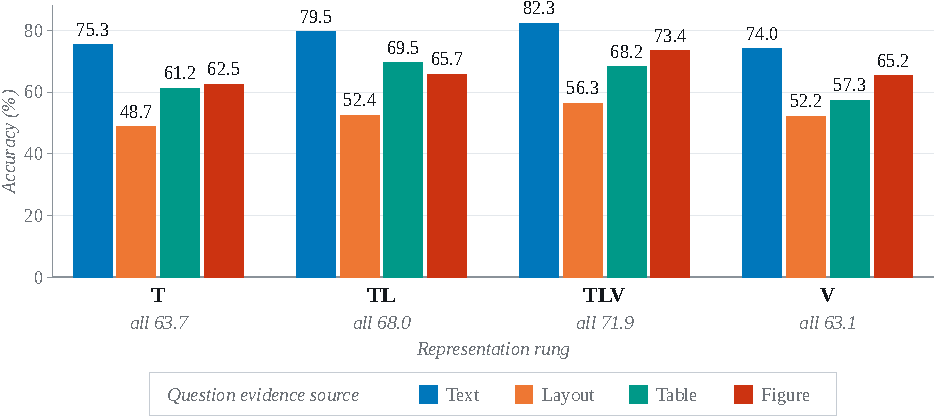
\includegraphics[width=0.8\columnwidth]{empirical/findings_figures/ladder_ldu_sources.pdf}
  \caption[LongDocURL accuracy by representation rung and evidence source]{LongDocURL accuracy by representation rung and evidence source. Evidence-source differences remain substantial across representation rungs.}
  \label{fig:ladder_ldu_sources}
\end{figure}

\paragraph{LongDocURL Replicates the Representation Pattern.} LongDocURL reproduces the same overall ordering, with \textbf{TLV} achieving the best pooled accuracy and outperforming the text-only rungs across every evidence source except tables (Figure~\ref{fig:ladder_ldu_sources}). The modality gap is weaker, however, because LongDocURL often exposes answer-relevant content directly through the document text layer even when the annotated evidence source is a figure or layout element. This helps explain why figure questions already reach 62.5\% at \textbf{T} and 65.7\% at \textbf{TL}, before rising to 73.4\% at \textbf{TLV}. The replication therefore supports the same underlying conclusion while showing that the apparent strength of a modality ceiling depends partly on dataset construction and how much visual evidence is redundantly recoverable from text.

\subsubsection{Conversion Fidelity}

% % Parser fidelity: text-only vs text+image accuracy for each text source,
% split digital / scanned. MMLongBench-Doc only.
% Teal = accuracy on a fixed [0,74] scale; warm = the vision gain (points).
% PyMuPDF reads the embedded text layer and runs no parser, so it is the baseline
% the three layout parsers are read against.
\definecolor{accteal}{HTML}{1BAF7A}
\definecolor{recwarm}{HTML}{D95926}
\newcommand{\pshade}[1]{%
  \pgfmathtruncatemacro{\shadeval}{max(0,min(60,(#1-0)/(74-0)*65))}%
  \edef\tmpcol{accteal!\shadeval}%
  \expandafter\cellcolor\expandafter{\tmpcol}%
}
\newcommand{\pcell}[1]{\pshade{#1}#1}
\newcommand{\gaincell}[1]{%
  \pgfmathtruncatemacro{\shadeval}{max(0,min(55,(#1-2)/(54-2)*55))}%
  \edef\tmpcol{recwarm!\shadeval}%
  \expandafter\cellcolor\expandafter{\tmpcol}$+$#1%
}

\begin{table}[ht]
\centering
\small
\setlength{\tabcolsep}{5pt}
\renewcommand{\arraystretch}{1.12}
\begin{tabular}{l rrr @{\hskip 10pt\vrule\hskip 10pt} rrr}
\toprule
 & \multicolumn{3}{c@{\hskip 10pt}}{\textbf{Digital}} & \multicolumn{3}{c}{\textbf{Scanned}} \\
\cmidrule(r){2-4}\cmidrule(l){5-7}
Text source & Text & $+$Image & $\Delta$ & Text & $+$Image & $\Delta$ \\
\midrule
PyMuPDF        & \pcell{40.6} & \pcell{49.7} & \gaincell{9.1} & \pcell{4.0}  & \pcell{57.7} & \gaincell{53.7} \\
PaddleOCR-VL   & \pcell{40.1} & \pcell{49.7} & \gaincell{9.6} & \pcell{32.8} & \pcell{61.2} & \gaincell{28.4} \\
MinerU 2.5     & \pcell{26.6} & \pcell{46.0} & \gaincell{19.3} & \pcell{27.4} & \pcell{55.7} & \gaincell{28.4} \\
Unlimited-OCR  & \pcell{42.3} & \pcell{50.2} & \gaincell{7.9} & \pcell{34.3} & \pcell{63.7} & \gaincell{29.4} \\
\midrule
Spread (max$-$min) & 15.6 & 4.2 & & 30.3 & 8.0 & \\
\bottomrule
\end{tabular}
\caption{Parser fidelity by text source and scan status. On MMLongBench-Doc. Adding the page image collapses the choice of parser: the spread across text sources falls from 30.3 points to 8.0 on scanned pages and from 15.6 to 4.2 on born-digital ones.}
\label{tab:parser}
\end{table}
\begin{figure}[ht]
  \centering
  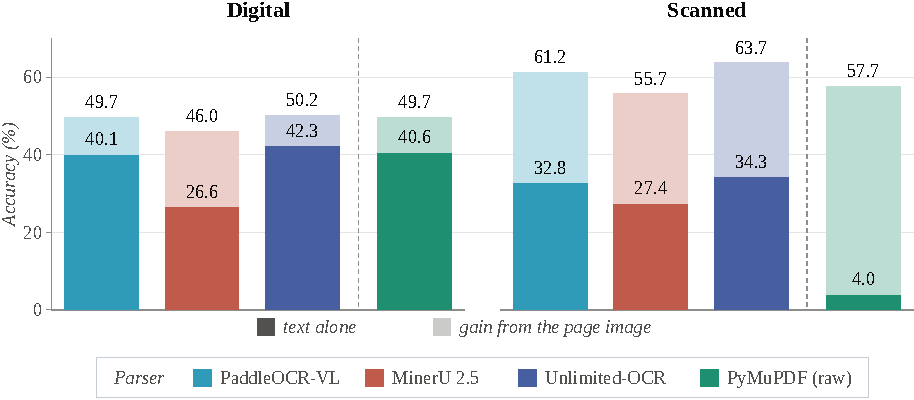
\includegraphics[width=0.7\columnwidth]{empirical/findings_figures/parser.pdf}
  \caption[Parser accuracy by text source]{Parser accuracy by text source with and without page images. Adding vision substantially reduces sensitivity to parser choice, particularly on scanned documents.}
  \label{fig:parser}
\end{figure}

\paragraph{Conversion Fidelity Constrains the Text Representation.} Parser choice changes only how the document is converted into text, yet produces substantial differences in downstream accuracy. This indicates that conversion fidelity is itself a representation bottleneck rather than a neutral preprocessing choice. MinerU produces the weakest parsed-text results on both digital and scanned documents, reaching 26.6\% and 27.4\%, compared with 40.1\% and 32.8\% for PaddleOCR-VL and 42.3\% and 34.3\% for Unlimited-OCR. The gap is especially revealing across document types. On born-digital pages, parsing mainly restructures or corrects an existing text layer, whereas on scanned pages it also determines whether a usable text representation is acquired at all. This is most extreme for PyMuPDF, where accuracy falls to 4.0\% on scans because the embedded text layer is often absent. In these cases, conversion failure does not merely degrade the representation but can remove the text channel entirely.

\paragraph{Vision Can Recover Conversion Errors.} Adding the page image substantially reduces the differences between parsers, showing that conversion loss can often be recovered when the original visual signal remains available. The spread between parsers falls from 15.7 points to 4.2 on digital documents and from 30.3 points to 8.0 on scanned documents. The weakest parser therefore benefits most from adding vision, indicating that many conversion errors are not irreversible once a second modality preserves the underlying signal. Information omitted or distorted during parsing can still be recovered directly from the page image, so the two channels provide partially redundant evidence. This redundancy reduces the extent to which parser quality constrains downstream performance. Conversion errors therefore become most damaging when no complementary channel retains the missing information.

% Resolution sweep by evidence source: low/med/high at the TLV and V rungs.
% Teal = accuracy on the shared ladder scale; warm = the low->high gain (points).
% Bold marks the best resolution in each row, within each rung block.
\definecolor{accteal}{HTML}{1BAF7A}
\definecolor{recwarm}{HTML}{D95926}
\newcommand{\rshade}[1]{%
  \pgfmathtruncatemacro{\shadeval}{max(0,min(60,(#1-14)/(74-14)*65))}%
  \edef\tmpcol{accteal!\shadeval}%
  \expandafter\cellcolor\expandafter{\tmpcol}%
}
\newcommand{\rcell}[1]{\rshade{#1}#1}
\newcommand{\rbest}[1]{\rshade{#1}\textbf{#1}}
\newcommand{\rgain}[1]{%
  \pgfmathtruncatemacro{\shadeval}{max(0,min(55,(#1-0)/(18-0)*55))}%
  \edef\tmpcol{recwarm!\shadeval}%
  \expandafter\cellcolor\expandafter{\tmpcol}$+$#1%
}

\begin{table}[ht]
\centering
\small
\setlength{\tabcolsep}{5pt}
\renewcommand{\arraystretch}{1.12}
\begin{tabular}{l rrrr @{\hskip 10pt\vrule\hskip 10pt} rrrr}
\toprule
 & \multicolumn{4}{c@{\hskip 10pt}}{\textbf{TLV}} & \multicolumn{4}{c}{\textbf{V}} \\
\cmidrule(r){2-5}\cmidrule(l){6-9}
Evidence source & low & med & high & $\Delta$ & low & med & high & $\Delta$ \\
\midrule
Chart            & \rcell{38.2} & \rcell{44.9} & \rbest{48.3} & \rgain{10.1} & \rcell{34.3} & \rcell{44.9} & \rbest{48.3} & \rgain{14.0} \\
Figure           & \rcell{39.7} & \rcell{45.5} & \rbest{48.3} & \rgain{8.6}  & \rcell{38.3} & \rcell{40.0} & \rbest{43.8} & \rgain{5.5} \\
Layout & \rcell{46.6} & \rcell{50.0} & \rbest{54.2} & \rgain{7.6}  & \rcell{47.5} & \rcell{49.2} & \rbest{53.4} & \rgain{5.9} \\
Text        & \rcell{52.9} & \rbest{55.0} & \rbest{55.0} & \rgain{2.1}  & \rcell{38.8} & \rcell{45.4} & \rbest{51.5} & \rgain{12.7} \\
Table            & \rcell{48.8} & \rbest{49.8} & \rcell{48.8} & \rgain{0.0}  & \rcell{25.3} & \rcell{37.3} & \rbest{42.4} & \rgain{17.1} \\
\midrule
\textbf{All}     & \rcell{49.2} & \rcell{52.5} & \rbest{54.7} & \rgain{5.5}  & \rcell{37.8} & \rcell{45.7} & \rbest{50.2} & \rgain{12.4} \\
\bottomrule
\end{tabular}
\caption{Render resolution by evidence source. On MMLongBench-Doc, at the TLV and V rungs. $\Delta$ indicates difference between high and low resolution.}
\label{tab:resolution_sweep}
\end{table}

\paragraph{Visual Fidelity Matters Most Without Textual Support.} Render resolution follows the same redundancy principle. Increasing resolution produces a much larger gain for \textbf{V} than for \textbf{TLV}, where accompanying text already preserves part of the fine-grained content that additional pixels would otherwise recover (Table~\ref{tab:resolution_sweep}). Low-resolution rendering is therefore most damaging when vision alone must carry small text, spatial detail, or other fine-grained visual evidence. Once those signals are redundantly represented in text, the marginal value of higher visual fidelity falls. Parser quality and render resolution thus expose the same mechanism from opposite sides: conversion errors matter most when they destroy the last usable representation of the required evidence.

\subsection{Selection}
\label{sec:findings_selection}

Selection determines which evidence reaches the reasoner. While both incomplete retrieval and irrelevant context are commonly treated as potential obstacles to long-document understanding~\citep{liu2025resolving,shi2023large,liu2024lost}, our results suggest that their effects are sharply asymmetric: incomplete coverage removes information that downstream stages cannot reliably recover, whereas irrelevant pages impose a comparatively smaller burden within the tested context range.

\subsubsection{Evidence Coverage}

\begin{figure}[h]
    \centering
    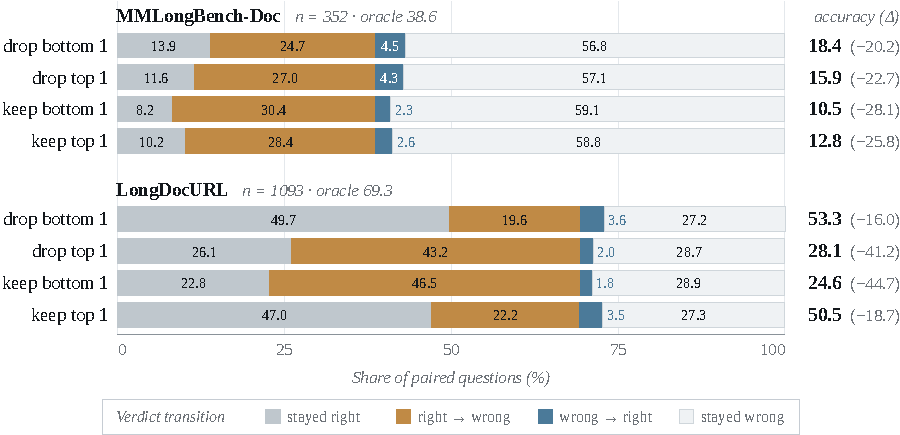
\includegraphics[width=0.9\columnwidth]{empirical/findings_figures/sufficiency.pdf}
    \caption[Verdict transitions under partial evidence coverage]{Verdict transitions after withholding or retaining gold evidence pages on MMLongBench-Doc and LongDocURL. Missing evidence predominantly converts correct answers into incorrect ones, while repairs are comparatively rare.}
    \label{fig:sufficiency}
\end{figure}

\begin{figure}[!h]
  \centering
  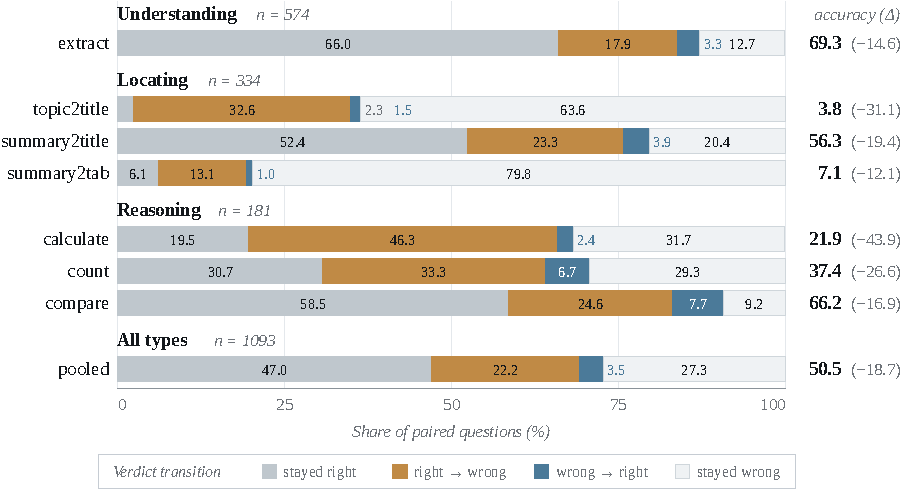
\includegraphics[width=0.9\columnwidth]{empirical/findings_figures/coverage_types.pdf}
    \caption[LongDocURL coverage sensitivity by question type]{LongDocURL verdict transitions under partial evidence coverage, grouped by question type. Extractive questions are relatively robust, while question types requiring evidence combination show substantially larger losses.}
  \label{fig:coverage_types}
\end{figure}

\paragraph{Evidence Coverage Is a Hard Constraint.} Our results confirm the field's expectation that incomplete evidence coverage strongly limits downstream performance. As Figure~\ref{fig:sufficiency} shows, removing required evidence overwhelmingly converts previously correct answers into incorrect ones, while the reverse transition is rare. On MMLongBench-Doc, withholding a single gold page changes 24.7--27.0\% of previously correct answers to incorrect, compared with only 4.3--4.5\% moving in the opposite direction. Retaining just one gold page widens this imbalance further, with 28.4--30.4\% changing from correct to incorrect and only 2.3--2.6\% being repaired. Missing evidence therefore places a hard constraint on downstream reasoning because information removed at selection cannot reliably be reconstructed later. Performance does not collapse completely, however, indicating that annotated multi-page questions are not always strictly dependent on every labelled page and may sometimes remain answerable from redundant evidence or information recoverable by the reasoner.

\paragraph{LongDocURL Replicates the Coverage Effect.} LongDocURL shows the same dependence on evidence coverage, although its annotations appear to contain more redundancy. Keeping only the highest-ranked gold page leaves 47.0\% of questions correct and retains 50.5\% accuracy, while dropping the highest-ranked gold page is substantially more damaging than dropping the lowest-ranked one. Figure~\ref{fig:coverage_types} explains much of this weaker pooled effect. \texttt{extract}, which dominates the benchmark, is comparatively robust because a single retained page often still contains the required answer span. In contrast, \texttt{calculate} questions require all necessary values to remain available, while \texttt{count} and \texttt{topic2title} more often depend on combining evidence across pages. LongDocURL therefore reproduces the coverage constraint, but the magnitude of the effect depends on whether the labelled pages are jointly necessary or partially redundant.

\subsubsection{Distractor Exposure}

% Adding distractor pages to a complete gold set, both datasets, k up to 5.
% Shading matches the withholding table. Both emit these \providecommand macros,
% so either table can be \input alone or first, in any order.
% Transition rows in the two-gold block pool questions with two and three gold
% pages. Cells beyond three distractors ran at TLV only on MMLongBench-Doc, and
% accuracy at the deeper counts is read on a shrinking pool under OOM attrition;
% the paired transition columns are unaffected.
\definecolor{accteal}{HTML}{1BAF7A}
\definecolor{recwarm}{HTML}{D95926}
\providecommand{\mshade}[1]{%
  \pgfmathtruncatemacro{\shadeval}{max(0,min(60,(#1-8)/(70-8)*65))}%
  \edef\tmpcol{accteal!\shadeval}\expandafter\cellcolor\expandafter{\tmpcol}}
\providecommand{\mcell}[1]{\mshade{#1}#1}
\providecommand{\mbest}[1]{\mshade{#1}\textbf{#1}}
\providecommand{\lshade}[1]{%
  \pgfmathtruncatemacro{\shadeval}{max(0,min(60,(#1-20)/(80-20)*65))}%
  \edef\tmpcol{accteal!\shadeval}\expandafter\cellcolor\expandafter{\tmpcol}}
\providecommand{\lcell}[1]{\lshade{#1}#1}
\providecommand{\lbest}[1]{\lshade{#1}\textbf{#1}}
\providecommand{\dmg}[1]{%
  \pgfmathtruncatemacro{\shadeval}{max(0,min(55,(#1)/48*55))}%
  \edef\tmpcol{recwarm!\shadeval}\expandafter\cellcolor\expandafter{\tmpcol}#1}
\providecommand{\rep}[1]{%
  \pgfmathtruncatemacro{\shadeval}{max(0,min(55,(#1)/48*55))}%
  \edef\tmpcol{accteal!\shadeval}\expandafter\cellcolor\expandafter{\tmpcol}#1}

\begin{table}[ht]
\centering
\small
\setlength{\tabcolsep}{3pt}
\renewcommand{\arraystretch}{1.12}
\begin{tabular}{l rrrr rr @{\hskip 6pt\vrule\hskip 6pt} rrrr rr}
\toprule
 & \multicolumn{6}{c@{\hskip 6pt}}{\textbf{MMLongBench-Doc}} & \multicolumn{6}{c}{\textbf{LongDocURL}} \\
\cmidrule(r){2-7}\cmidrule(l){8-13}
Condition & T & TL & TLV & V & R$\rightarrow$W & W$\rightarrow$R & T & TL & TLV & V & R$\rightarrow$W & W$\rightarrow$R \\
\midrule
\multicolumn{13}{@{}l}{\emph{1 gold page}} \\
Oracle           & \mcell{37.1} & \mcell{44.6} & \mbest{63.7} & \mcell{55.0} & --- & --- & \lcell{65.6} & \lcell{74.0} & \lbest{74.7} & \lcell{64.5} & --- & --- \\
$+$1 distractor  & \mcell{39.5} & \mcell{48.9} & \mbest{63.7} & \mcell{55.7} & \dmg{7.8} & \rep{7.0} & \lcell{65.4} & \lcell{72.4} & \lbest{74.4} & \lcell{63.0} & \dmg{8.5} & \rep{8.1} \\
$+$2 distractors & \mcell{38.8} & \mcell{47.9} & \mbest{64.3} & \mcell{56.1} & \dmg{8.2} & \rep{8.0} & \lcell{65.1} & \lcell{68.7} & \lbest{72.0} & \lcell{63.9} & \dmg{9.3} & \rep{7.5} \\
$+$3 distractors & \mcell{40.9} & \mcell{47.0} & \mbest{63.1} & \mcell{55.1} & \dmg{9.7} & \rep{8.2} & \lcell{64.5} & \lcell{68.0} & \lbest{68.4} & \lcell{62.1} & \dmg{11.7} & \rep{6.9} \\
$+$4 distractors & \mcell{41.9} & \mcell{45.3} & \mbest{62.5} & \mcell{52.5} & \dmg{9.5} & \rep{6.6} & \lcell{63.5} & \lcell{68.0} & \lbest{72.2} & \lcell{62.5} & \dmg{10.5} & \rep{8.7} \\
$+$5 distractors & \mcell{39.5} & \mcell{42.6} & \mbest{62.3} & \mcell{54.4} & \dmg{10.0} & \rep{6.9} & \lcell{64.6} & \lcell{69.1} & \lbest{70.2} & \lcell{60.8} & \dmg{11.4} & \rep{7.3} \\
\addlinespace
\multicolumn{13}{@{}l}{\emph{2 gold pages}} \\
Oracle           & \mcell{28.9} & \mcell{33.3} & \mbest{37.8} & \mcell{34.6} & --- & --- & \lcell{62.2} & \lcell{63.4} & \lbest{70.4} & \lcell{61.5} & --- & --- \\
$+$1 distractor  & \mcell{25.7} & \mcell{34.0} & \mbest{38.6} & \mcell{34.4} & \dmg{7.8} & \rep{7.5} & \lcell{58.7} & \lcell{63.0} & \lbest{66.2} & \lcell{57.9} & \dmg{9.6} & \rep{4.1} \\
$+$2 distractors & \mcell{25.3} & \mcell{33.6} & \mbest{35.7} & \mcell{32.4} & \dmg{9.6} & \rep{6.0} & \lcell{58.9} & \lcell{62.2} & \lbest{66.4} & \lcell{57.4} & \dmg{10.9} & \rep{4.4} \\
$+$3 distractors & \mcell{21.6} & \mcell{28.2} & \mbest{33.6} & \mcell{33.2} & \dmg{11.4} & \rep{6.0} & \lcell{58.1} & \lcell{63.3} & \lbest{70.8} & \lcell{57.8} & \dmg{9.7} & \rep{6.0} \\
$+$4 distractors & \mcell{24.6} & \mcell{30.7} & \mbest{43.7} & \mcell{31.3} & \dmg{11.8} & \rep{11.8} & \lcell{57.8} & \lcell{63.2} & \lbest{68.3} & \lcell{57.1} & \dmg{13.3} & \rep{6.1} \\
% $+$5 distractors & \mcell{20.5} & \mcell{29.5} & \mbest{44.7} & \mcell{32.1} & \dmg{10.6} & \rep{8.2} & \lcell{56.4} & \lcell{61.5} & \lbest{69.0} & \lcell{54.9} & \dmg{12.6} & \rep{5.9} \\
\bottomrule
\end{tabular}
\caption{Adding distractor pages to a complete gold set. Distractors ranked by ColQwen3 and verdict transitions indicate the proportion of questions that turned incorrect when previously correct or vice versa when distractors were added at the \textbf{TLV} rung.}
\label{tab:exposure}
\end{table}

\paragraph{Distractor Exposure Is Comparatively Harmless.} Our results challenge the common concern that longer contexts necessarily degrade evidence use. Prior work on \emph{lost in the middle} and related long-context effects shows that models can struggle when relevant information is buried among competing tokens, particularly as context length grows~\citep{liu2024lost}. In our setting, however, adding up to five distractor pages produces only modest changes. At \textbf{TLV}, single-page MMLongBench-Doc questions remain essentially stable, while two-page questions show a larger but still gradual decline as additional distractors are introduced. The verdict transitions show that distractors break some answers but also repair others, suggesting that they perturb evidence discrimination rather than simply remove usable information. The tested range is also practically bounded by the hardware available for multimodal inference. Within these realistic page budgets, preserving recall appears more important than aggressively removing irrelevant evidence.

\paragraph{The Remaining Distractor Cost Appears to Be a Reasoning Problem.} LongDocURL strengthens this interpretation. Its two-page questions do not show the same decline despite receiving the same number of additional pages, making a pure attention-dilution explanation less likely. As established in the representation analysis, LongDocURL is also substantially easier overall than MMLongBench-Doc across representation rungs, suggesting that its questions leave more margin before distractors begin to affect reasoning. A more plausible explanation is that the harder MMLongBench-Doc questions are therefore more sensitive to small increases in reasoning burden once irrelevant evidence is introduced. This distinction is important for retrieval design. Distractor-induced failures may be recoverable through stronger reasoning or evidence-selection interventions, whereas omitted evidence cannot be reconstructed once it is absent from the context. 
% Retrieval can therefore favour recall over precision within the tested range, accepting moderate distractor exposure to reduce the more fundamental risk of missing required evidence.

\subsection{Reasoning}
\label{sec:findings_reasoning}

Reasoning determines whether the supplied evidence is correctly combined and interpreted to produce an answer. Even when representation preserves the required information and selection delivers it to the reasoner, failures can still arise at this final stage. Our results identify two recurring limitations: current models struggle to integrate evidence distributed across pages, and they do not reliably distinguish genuinely insufficient evidence from difficult but answerable cases.

\subsubsection{Evidence Integration}

% Integration by evidence source at the TLV rung, both datasets side by side.
% Teal = accuracy on a per-dataset scale; warm wash on M-S deepens with the deficit,
% over [0, 38] points.
% Source rows OVERLAP: a question citing Chart and Table is counted in both, so the
% rows are blocks and the All row pools each question once rather than summing them.
% Multi is derived from the 2 and 3+ buckets and their n, so the buckets reproduce it.
% Read the 3+ column for trend: crossed with five sources it thins out, to n=20 on
% Chart and n=12 on Table.
\definecolor{gapred}{HTML}{B03A2E}
\definecolor{accteal}{HTML}{1BAF7A}
\newcommand{\kshade}[1]{%
  \pgfmathtruncatemacro{\shadeval}{max(0,min(60,(#1-14)/(70-14)*65))}%
  \edef\tmpcol{accteal!\shadeval}\expandafter\cellcolor\expandafter{\tmpcol}}
\newcommand{\kcell}[1]{\kshade{#1}#1}
\newcommand{\nshade}[1]{%
  \pgfmathtruncatemacro{\shadeval}{max(0,min(60,(#1-40)/(88-40)*65))}%
  \edef\tmpcol{accteal!\shadeval}\expandafter\cellcolor\expandafter{\tmpcol}}
\newcommand{\ncell}[1]{\nshade{#1}#1}

\begin{table}[ht]
\centering
\small
\setlength{\tabcolsep}{4pt}
\renewcommand{\arraystretch}{1.12}
\begin{tabular}{@{}l rrr rr @{\hskip 6pt\vrule\hskip 6pt} l rrr rr@{}}
\toprule
\multicolumn{6}{c@{\hskip 6pt}}{\textbf{MMLongBench-Doc}} & \multicolumn{6}{c}{\textbf{LongDocURL}} \\
\cmidrule(r){1-6}\cmidrule(l){7-12}
 & \multicolumn{3}{c}{Gold pages} & \multicolumn{2}{c@{\hskip 6pt}}{Pooled} & & \multicolumn{3}{c}{Gold pages} & \multicolumn{2}{c}{Pooled} \\
\cmidrule(lr){2-4}\cmidrule(lr){5-6}\cmidrule(lr){8-10}\cmidrule(lr){11-12}
\textbf{Evidence source} & \textbf{1} & \textbf{2} & \textbf{3+} & \textbf{Multi} & \textbf{M$-$S} & \textbf{Evidence source} & \textbf{1} & \textbf{2} & \textbf{3+} & \textbf{Multi} & \textbf{M$-$S} \\
\midrule
Chart            & \kcell{58.2} & \kcell{32.2} & \kcell{15.0} & \kcell{27.8} & \cellcolor{gapred!36}$-$30.4 & ---    &              &              &              &              &              \\
Figure           & \kcell{49.4} & \kcell{34.3} & \kcell{44.9} & \kcell{38.7} & \cellcolor{gapred!13}$-$10.7 & Figure & \ncell{68.4} & \ncell{84.3} & \ncell{63.3} & \ncell{79.3} & \cellcolor{gapred!13}$+$10.9 \\
Layout & \kcell{64.3} & \kcell{44.1} & \kcell{34.6} & \kcell{40.0} & \cellcolor{gapred!29}$-$24.3 & Layout & \ncell{63.1} & \ncell{52.5} & \ncell{58.1} & \ncell{54.0} & \cellcolor{gapred!11}$-$9.1 \\
Text        & \kcell{66.2} & \kcell{44.7} & \kcell{40.0} & \kcell{43.3} & \cellcolor{gapred!27}$-$22.9 & Text   & \ncell{82.3} & \ncell{85.2} & \ncell{73.9} & \ncell{82.3} & \cellcolor{gapred!0}0.0 \\
Table            & \kcell{69.2} & \kcell{31.6} & \kcell{41.7} & \kcell{32.7} & \cellcolor{gapred!43}$-$36.5 & Table  & \ncell{75.4} & \ncell{52.2} & \ncell{42.3} & \ncell{51.1} & \cellcolor{gapred!29}$-$24.3 \\
\midrule
\textbf{All}     & \kcell{63.7} & \kcell{37.8} & \kcell{38.4} & \kcell{38.0} & \cellcolor{gapred!30}$-$25.7 & \textbf{All} & \ncell{74.7} & \ncell{70.4} & \ncell{65.2} & \ncell{69.2} & \cellcolor{gapred!6}$-$5.5 \\
\bottomrule
\end{tabular}
\caption{Accuracy by gold-page count and evidence source at the \textbf{TLV} rung. The single- to multi-page deficit varies substantially by evidence type, indicating that integration difficulty depends on what evidence must be combined as well as where it is located.}
\label{tab:integration_sources}
\end{table}
% % GENERATED by tables/scripts/ -- do not edit by hand, re-run the script.
% Numbers read from results/tables/mmlongbench/*.csv.
% mmlongbench/mmlb_within_page, longdocurl/ldu_true_multihop
% Shade ranges are fitted to the values present:
% Accuracy: accteal over [18.2, 74.5]  % Difference from the group's 1-page row: recwarm over [-40.9, -2.4]
\definecolor{accteal}{HTML}{1BAF7A}
\definecolor{recwarm}{HTML}{D95926}
\begin{table}[ht]
\centering
\small
\setlength{\tabcolsep}{5pt}
\adjustbox{max width=\textwidth}{%
\begin{tabular}{l@{\hskip 14pt}rrrr@{\hskip 14pt}rrrr}
\toprule
 & \multicolumn{4}{c}{\textbf{Accuracy}} & \multicolumn{4}{c}{\textbf{Difference from the group's 1-page row}} \\
\cmidrule(lr){2-5} \cmidrule(lr){6-9}
\textbf{Evidence spread} & \textbf{T} & \textbf{TL} & \textbf{TLV} & \textbf{V} & \textbf{T} & \textbf{TL} & \textbf{TLV} & \textbf{V} \\
\midrule
\multicolumn{9}{l}{\emph{MMLongBench-Doc}} \\
1 page, 1 source & \cellcolor{accteal!25}41.5 & \cellcolor{accteal!30}46.7 & \cellcolor{accteal!51}66.2 & \cellcolor{accteal!44}59.6 & -- & -- & -- & -- \\
1 page, 2+ sources & \cellcolor{accteal!0}18.2 & \cellcolor{accteal!15}32.7 & \cellcolor{accteal!32}\textbf{48.2} & \cellcolor{accteal!19}36.4 & \cellcolor{recwarm!33}\textbf{-23.3} & \cellcolor{recwarm!18}-14.0 & \cellcolor{recwarm!24}-18.0 & \cellcolor{recwarm!33}-23.3 \\
2+ pages, 1 source & \cellcolor{accteal!9}\textbf{26.3} & \cellcolor{accteal!17}\textbf{34.4} & \cellcolor{accteal!25}42.0 & \cellcolor{accteal!20}\textbf{37.1} & \cellcolor{recwarm!20}-15.1 & \cellcolor{recwarm!15}-12.3 & \cellcolor{recwarm!34}-24.2 & \cellcolor{recwarm!31}-22.6 \\
2+ pages, 2+ sources & \cellcolor{accteal!7}24.4 & \cellcolor{accteal!10}27.6 & \cellcolor{accteal!18}35.0 & \cellcolor{accteal!12}29.3 & \cellcolor{recwarm!23}-17.1 & \cellcolor{recwarm!26}\textbf{-19.1} & \cellcolor{recwarm!45}\textbf{-31.2} & \cellcolor{recwarm!43}\textbf{-30.3} \\
\addlinespace
\multicolumn{9}{l}{\emph{LongDocURL}} \\
1 page & \cellcolor{accteal!50}65.5 & \cellcolor{accteal!59}73.8 & \cellcolor{accteal!60}74.5 & \cellcolor{accteal!49}64.4 & -- & -- & -- & -- \\
2+ pages, all types & \cellcolor{accteal!47}\textbf{62.2} & \cellcolor{accteal!47}\textbf{62.4} & \cellcolor{accteal!54}\textbf{69.3} & \cellcolor{accteal!47}\textbf{62.0} & \cellcolor{recwarm!1}-3.3 & \cellcolor{recwarm!14}-11.4 & \cellcolor{recwarm!5}-5.3 & \cellcolor{recwarm!0}-2.4 \\
2+ pages, multi-hop types only & \cellcolor{accteal!21}37.5 & \cellcolor{accteal!16}33.0 & \cellcolor{accteal!24}40.3 & \cellcolor{accteal!19}36.4 & \cellcolor{recwarm!40}\textbf{-28.0} & \cellcolor{recwarm!60}\textbf{-40.9} & \cellcolor{recwarm!50}\textbf{-34.2} & \cellcolor{recwarm!40}\textbf{-28.0} \\
\bottomrule
\end{tabular}%
}

\caption{\small Accuracy by how a question's evidence is spread. Oracle pages, uninstructed. LongDocURL's mild integration deficit is an artifact of its annotation: restricted to the question types that genuinely need several pages, it goes from $-$5.3 to $-$34.2 at TLV and becomes the larger of the two corpora. MMLongBench-Doc pays almost as much for a second evidence source on one page as for a second page.}
\label{tab:integration_multihop}
\end{table}
% {\footnotesize\raggedright
% Judge-scored accuracy (\%), uninstructed prompt, oracle pages. The difference block is each
% row minus its own group's one-page row, in points, so the two corpora are each read against
% themselves. Bold is the largest accuracy and the largest deficit in each column; the two
% baseline rows take no part in either contest.
% \textbf{The row sets differ because the two annotations fail differently.} MMLongBench-Doc's
% rows cross the gold-page count with the number of distinct evidence sources cited: 105 of its
% 480 one-page questions cite two or more, so they ask the reasoner to combine a chart with a
% caption or a table with its surrounding text while the \texttt{hop} label still calls them
% single-page. Reading the deficit against the clean \emph{1 page, 1 source} row rather than
% against all one-page questions widens it from $-$25.0 to $-$28.7 at TLV.
% LongDocURL's \texttt{evidence\_pages} instead records every page the evidence is \emph{visible}
% on rather than the pages an answer \emph{needs}, so a fact repeated across pages is labelled
% multi-page. Of the multi-page questions the reasoner solves with the whole gold set, 67.9\%
% are still solved from the top-ranked gold page alone. The last row keeps only the question
% types where that share is under half (\texttt{topic2title}, \texttt{summary2tab},
% \texttt{calculate}, \texttt{count}), which is where the corpus asks for integration at all.
% Both cuts are observational: these are question populations, not one population under a
% treatment, so a difference carries whatever else separates them.\par}


\begin{figure}[!h]
  \centering
  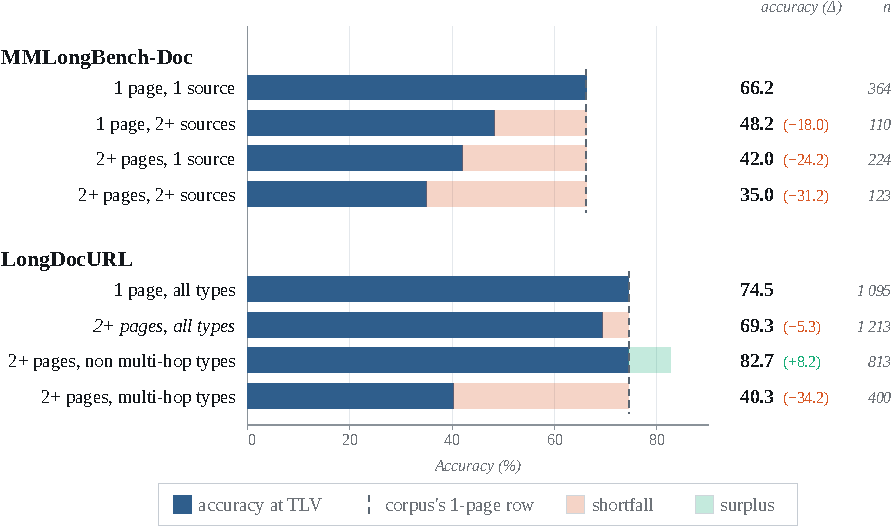
\includegraphics[width=0.8\columnwidth]{empirical/findings_figures/integration_multihop.pdf}
  \caption[Accuracy by multi-hop evidence structure]{Accuracy by multi-hop evidence structure at the \textbf{TLV} rung. MMLongBench-Doc accuracy declines as evidence must be combined across additional sources and pages, while LongDocURL shows a large deficit only for question types established as genuinely multi-hop.}
  \label{fig:integration_multihop}
\end{figure}

\paragraph{Cross-Page Integration Adds a Distinct Reasoning Burden.} Our results show that questions requiring evidence from several pages remain substantially harder even when all annotated evidence is supplied. As shown in Figure~\ref{fig:integration_multihop}, MMLongBench-Doc \textbf{TLV} accuracy falls from 66.2\% for single-page, single-source questions to 42.0\% when a single evidence source spans multiple pages, and to 35.0\% when multiple sources are also involved. Because its gold pages largely form a minimal evidence set, these multi-page questions generally require several pieces of evidence to be combined. Since oracle pages are supplied, the deficit arises after the required evidence has already reached the reasoner. LongDocURL shows a much smaller pooled deficit because many nominally multi-page questions remain answerable from a single retained page.

\paragraph{Multi-Hop Integration Drives the MMLongBench-Doc Deficit.} Table~\ref{tab:integration_sources} further supports this interpretation by showing that the multi-page deficit varies substantially with the evidence being combined. Questions involving tables and charts show some of the largest declines, consistent with the additional burden of recovering and relating several structured pieces of evidence. The difficulty therefore appears to arise primarily from the integration operation required by the question rather than from page count alone.

\paragraph{LongDocURL Shows the Same Deficit on Genuinely Multi-Hop Questions.} As established in the evidence-coverage analysis, \texttt{topic2title}, \texttt{summary2tab}, \texttt{calculate}, and \texttt{count} are the LongDocURL question types that are genuinely multi-hop because they become substantially less answerable when only the highest-ranked gold page is retained. Figure~\ref{fig:integration_multihop} shows that these types fall to 40.3\% on multi-page questions, a 34.2-point deficit relative to the single-page baseline, while the remaining multi-page types reach 82.7\%. LongDocURL therefore exhibits the same integration bottleneck once the analysis focuses on questions that genuinely require multiple pieces of evidence.

% \begin{figure}[p]
%   \centering
%   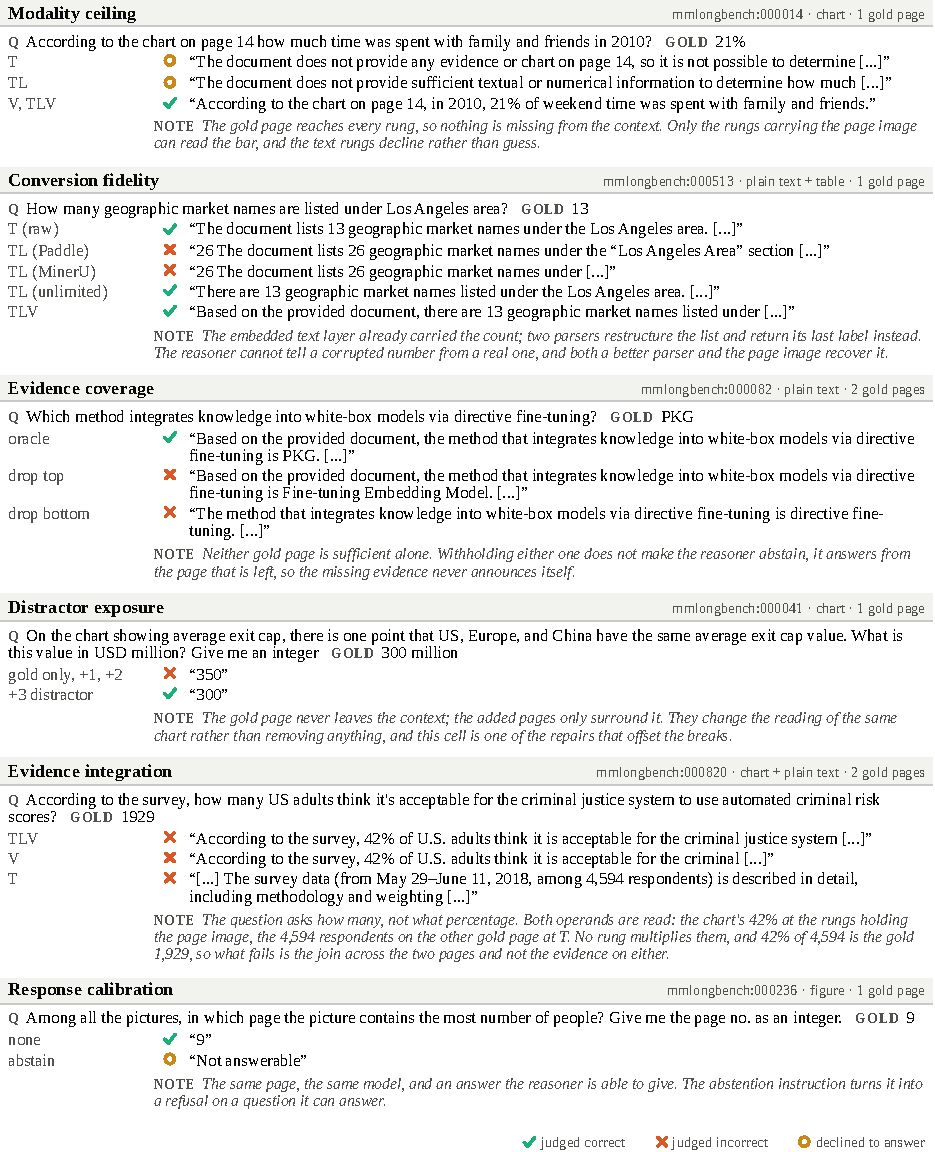
\includegraphics[width=\columnwidth]{empirical/findings_figures/worked_examples.pdf}
%   \caption[Worked examples of the six failure mechanisms]{Worked examples of the six failure mechanisms, one question each, from MMLongBench-Doc under Qwen3-VL-8B. Every band gives the question, its gold answer, and what the reasoner returned under each condition that mechanism is tested by, marked with the judge's verdict; the quotations are the model's own output, elided at [\ldots]. The annotated gold pages are supplied in every condition except \emph{drop top} and \emph{drop bottom}, so a wrong answer anywhere else is not a coverage failure, and the conditions are named as \S\ref{sec:emp_methodology} defines them. Each example is reproducible from its question id.}
%   \label{fig:worked_examples}
% \end{figure}


\subsubsection{Response Calibration}

\begin{figure}[h]
  \centering
  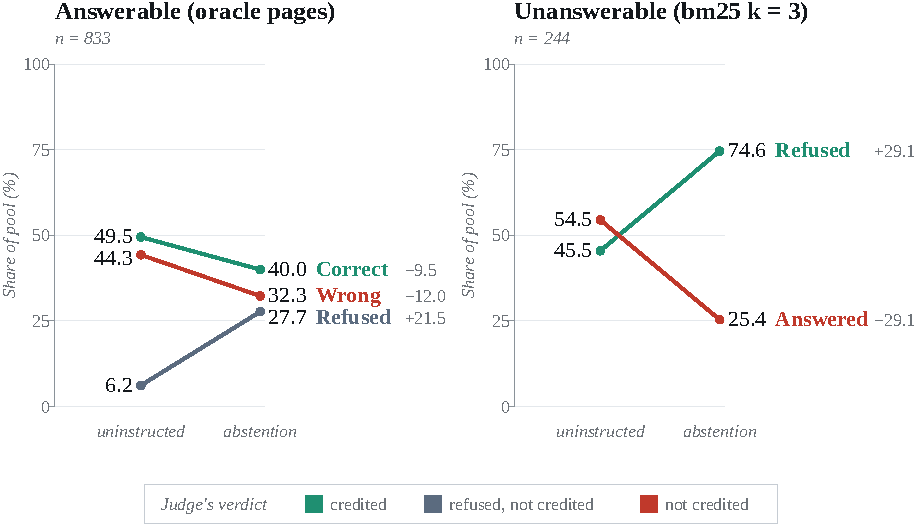
\includegraphics[width=0.7\columnwidth]{empirical/findings_figures/abstention_outcomes.pdf}
  \caption[Effect of abstention prompting on answerable and unanswerable questions]{Effect of targeted abstention prompting at the \textbf{TLV} rung. The instruction reduces unsupported answering when evidence is insufficient, but also increases refusal on answerable questions.}
  \label{fig:abstention_outcomes}
\end{figure}

\paragraph{The Reasoner Does Not Reliably Calibrate Evidence Sufficiency.} Figure~\ref{fig:abstention_outcomes} shows that targeted abstention prompting at the \textbf{TLV} rung makes the reasoner substantially more conservative, but not selectively so. On unanswerable questions, refusal rises from 45.5\% to 74.6\%, substantially reducing unsupported answers. The same intervention also raises refusal on answerable questions from 6.2\% to 27.7\%, while correct answers fall from 49.5\% to 40.0\%. Incorrect answers decline as well, indicating that the prompt suppresses some unreliable responses, but it does so by shifting the model towards refusal rather than by improving its ability to distinguish sufficient from insufficient evidence. The reasoner therefore remains poorly calibrated between cases where evidence is genuinely absent and cases where the available evidence is simply difficult to interpret.

% GENERATED by tables/scripts/ -- do not edit by hand, re-run the script.
% Numbers read from results/tables/analysis/*.csv.
% analysis/faithfulness_answerable_accuracy_source (results.errcat.jsonl)
% Shade ranges are fitted to the values present:
% Acc.: accteal over [26.4, 51.0]  % Abst.: neutral over [0.8, 35.5]  % Inc.: recwarm over [30.3, 50.0]
\definecolor{accteal}{HTML}{1BAF7A}
\definecolor{neutral}{HTML}{5B6B7F}
\definecolor{recwarm}{HTML}{D95926}
\definecolor{ngray}{HTML}{7A8494}
\begin{table}[ht]
\centering
\small
\setlength{\tabcolsep}{5pt}
\renewcommand{\arraystretch}{1.12}
\begin{tabular}{@{}l r rrr @{\hskip 10pt} rrr@{}}
\toprule
 & & \multicolumn{3}{c}{\textbf{No instruction}} & \multicolumn{3}{c}{\textbf{Abstention instruction}} \\
\cmidrule(lr){3-5}\cmidrule(l){6-8}
\textbf{Evidence source} & \textcolor{ngray}{\scriptsize$n$} & \textbf{Acc.} & \textbf{Abst.} & \textbf{Inc.} & \textbf{Acc.} & \textbf{Abst.} & \textbf{Inc.} \\
\midrule
Text & \textcolor{ngray}{\scriptsize286} & \cellcolor{accteal!60}\textbf{51.0} & \cellcolor{neutral!11}7.3 & \cellcolor{recwarm!34}41.6 & \cellcolor{accteal!42}\textbf{43.7} & \cellcolor{neutral!40}24.1 & \cellcolor{recwarm!6}32.2 \\
Layout & \textcolor{ngray}{\scriptsize118} & \cellcolor{accteal!56}49.2 & \cellcolor{neutral!0}\textbf{0.8} & \cellcolor{recwarm!60}\textbf{50.0} & \cellcolor{accteal!37}41.5 & \cellcolor{neutral!32}\textbf{19.5} & \cellcolor{recwarm!26}39.0 \\
Table & \textcolor{ngray}{\scriptsize208} & \cellcolor{accteal!45}44.7 & \cellcolor{neutral!10}6.7 & \cellcolor{recwarm!56}48.6 & \cellcolor{accteal!30}38.5 & \cellcolor{neutral!51}30.3 & \cellcolor{recwarm!3}31.2 \\
Chart & \textcolor{ngray}{\scriptsize178} & \cellcolor{accteal!40}42.7 & \cellcolor{neutral!11}7.3 & \cellcolor{recwarm!60}\textbf{50.0} & \cellcolor{accteal!0}26.4 & \cellcolor{neutral!42}25.3 & \cellcolor{recwarm!55}\textbf{48.3} \\
Figure & \textcolor{ngray}{\scriptsize290} & \cellcolor{accteal!39}42.4 & \cellcolor{neutral!12}7.6 & \cellcolor{recwarm!60}\textbf{50.0} & \cellcolor{accteal!19}34.1 & \cellcolor{neutral!60}35.5 & \cellcolor{recwarm!0}30.3 \\
\midrule
\emph{All} & \textcolor{ngray}{\scriptsize833} & \cellcolor{accteal!56}49.5 & \cellcolor{neutral!9}6.2 & \cellcolor{recwarm!43}44.3 & \cellcolor{accteal!33}40.0 & \cellcolor{neutral!47}27.7 & \cellcolor{recwarm!6}32.3 \\
\bottomrule
\end{tabular}
\caption{Refusal outcomes by evidence source under targeted abstention prompting at \textbf{TLV}. False abstention is more frequent for visually and structurally demanding evidence, suggesting that reasoning difficulty influences the decision to refuse.}
\label{tab:abstention_sources}
\end{table}


\paragraph{Reasoning Difficulty Is Mistaken for Evidence Insufficiency.} Table~\ref{tab:abstention_sources} supports this interpretation by showing that false abstention varies with the evidence being reasoned over. Under the abstention instruction, refusal reaches 35.5\% for figure questions and 30.3\% for table questions, compared with 25.3\% for charts and 24.1\% for text. Since all questions are evaluated with oracle pages and the full \textbf{TLV} representation, these differences cannot be explained by missing evidence. Instead, the model appears increasingly willing to abstain as interpretation becomes more difficult, suggesting that reasoning difficulty is being treated as evidence insufficiency. Response calibration therefore remains coupled to reasoning confidence rather than to whether the required evidence is actually present.
\section{Error Analysis}
\label{sec:emp_error_analysis}

The error taxonomy provides a finer view of how the reasoner fails once representation and evidence selection are controlled. Unlike the preceding analyses, each category is reported as a share of the full question pool for that condition, allowing direct comparison across prompt modes, evidence sources, and evidence-page counts. 
Since the abstention trade-off has already been analysed in \S\ref{sec:findings_reasoning}, we do not revisit the \texttt{abstain} variants here and instead focus on the remaining prompt behaviours and error shifts.

\subsection{Prompt Mode Analysis}

% % GENERATED by tables/scripts/ -- do not edit by hand, re-run the script.
% Numbers read from results/tables/analysis/*.csv.
% error_profile_prompt, error_profile_prompt_unanswerable (results.errcat.jsonl)
% Shade ranges are fitted to the values present:
% Share of the pool, at TLV (\%): recwarm over [0.0, 60.0]
\definecolor{recwarm}{HTML}{D95926}
\begin{table*}[h]
\centering
\small
\setlength{\tabcolsep}{5pt}
\adjustbox{max width=\textwidth}{%
\begin{tabular}{l@{\hskip 14pt}rrrrrr}
\toprule
 & \multicolumn{6}{c}{\textbf{Share of the pool, at TLV (\%)}} \\
\cmidrule(lr){2-7}
\textbf{Error category} & \textbf{none} & \textbf{grounded} & \textbf{abstain} & \textbf{abstain\_bal.} & \textbf{cot} & \textbf{extract\_cot} \\
\midrule
\multicolumn{7}{l}{\emph{answerable pool (oracle pages)}} \\
insufficient evidence & \cellcolor{recwarm!6}6.1 & \cellcolor{recwarm!6}6.0 & \cellcolor{recwarm!28}\textbf{27.6} & \cellcolor{recwarm!23}\textbf{23.0} & \cellcolor{recwarm!7}6.6 & \cellcolor{recwarm!9}8.8 \\
no answer reached & \cellcolor{recwarm!7}6.8 & \cellcolor{recwarm!0}0.0 & \cellcolor{recwarm!0}0.0 & \cellcolor{recwarm!0}0.0 & \cellcolor{recwarm!4}4.4 & \cellcolor{recwarm!3}3.3 \\
equivocal & \cellcolor{recwarm!1}1.1 & \cellcolor{recwarm!0}0.1 & \cellcolor{recwarm!0}0.0 & \cellcolor{recwarm!0}0.0 & \cellcolor{recwarm!0}0.0 & \cellcolor{recwarm!0}0.1 \\
wrong count & \cellcolor{recwarm!14}\textbf{14.4} & \cellcolor{recwarm!19}\textbf{18.8} & \cellcolor{recwarm!11}10.9 & \cellcolor{recwarm!12}11.8 & \cellcolor{recwarm!15}\textbf{14.8} & \cellcolor{recwarm!13}\textbf{12.7} \\
wrong value & \cellcolor{recwarm!9}9.0 & \cellcolor{recwarm!15}14.6 & \cellcolor{recwarm!9}8.8 & \cellcolor{recwarm!11}10.8 & \cellcolor{recwarm!8}8.5 & \cellcolor{recwarm!10}10.1 \\
wrong entity & \cellcolor{recwarm!8}7.7 & \cellcolor{recwarm!10}9.6 & \cellcolor{recwarm!7}7.1 & \cellcolor{recwarm!7}7.3 & \cellcolor{recwarm!7}7.1 & \cellcolor{recwarm!9}8.7 \\
incomplete list & \cellcolor{recwarm!2}1.8 & \cellcolor{recwarm!3}2.6 & \cellcolor{recwarm!2}1.9 & \cellcolor{recwarm!2}2.0 & \cellcolor{recwarm!3}2.9 & \cellcolor{recwarm!2}2.2 \\
over-inclusive list & \cellcolor{recwarm!2}2.2 & \cellcolor{recwarm!3}2.8 & \cellcolor{recwarm!2}2.0 & \cellcolor{recwarm!2}2.5 & \cellcolor{recwarm!3}2.9 & \cellcolor{recwarm!3}3.4 \\
unit / format mismatch & \cellcolor{recwarm!1}1.3 & \cellcolor{recwarm!2}1.6 & \cellcolor{recwarm!1}1.4 & \cellcolor{recwarm!1}1.3 & \cellcolor{recwarm!2}2.3 & \cellcolor{recwarm!2}2.3 \\
other & \cellcolor{recwarm!0}0.1 & \cellcolor{recwarm!0}0.1 & \cellcolor{recwarm!0}0.1 & \cellcolor{recwarm!0}0.1 & \cellcolor{recwarm!0}0.4 & \cellcolor{recwarm!1}0.8 \\
\emph{All incorrect} & \cellcolor{recwarm!50}50.5 & \cellcolor{recwarm!56}56.3 & \cellcolor{recwarm!60}60.0 & \cellcolor{recwarm!59}59.1 & \cellcolor{recwarm!50}49.8 & \cellcolor{recwarm!52}52.5 \\
\bottomrule
\end{tabular}%
}

\vspace{2pt}
% {\footnotesize\raggedright
% Rung \textbf{TLV}, judged under the error-taxonomy rubric. The denominator is each column's
% scored questions (its $n$), which excludes OOM cells: those carry no answer, so they are
% neither a right answer nor a kind of wrong one. Categories are assigned first-match-wins in a
% fixed priority order, so they are mutually exclusive and every incorrect answer lands in
% exactly one; \emph{All incorrect} is their sum and equals 100 minus that column's accuracy.
% Bold is the largest value in each column within a group, the totals excepted.
% \textbf{The two groups are not comparable in level.} The answerable pool runs on oracle pages
% and the unanswerable pool on the bm25 $k{=}3$ page set, because an unanswerable question has
% no gold page to select. \emph{answered unanswerable} appears only in the second group: on a
% pool with an answer it can only be the judge misapplying the label, and on a pool without one
% it is the entire error, which is why \emph{All incorrect} reproduces it there.
% \emph{no answer reached} is a response that reasoned without committing, typically one that
% exhausted its decode budget mid-calculation; it is absent under the three modes that ask for
% a short answer. Read the answerable group beside Table~\ref{tab:prompting}, whose accuracies
% are what these rates decompose.\par}
\caption{\small Failure modes under six prompt instructions. Each cell is the share of that column's own question pool assigned the category, so a group's rows sum to its \emph{All incorrect} row rather than to 100.}
\label{tab:error_profile}
\end{table*}

\begin{figure}[H]
  \centering
  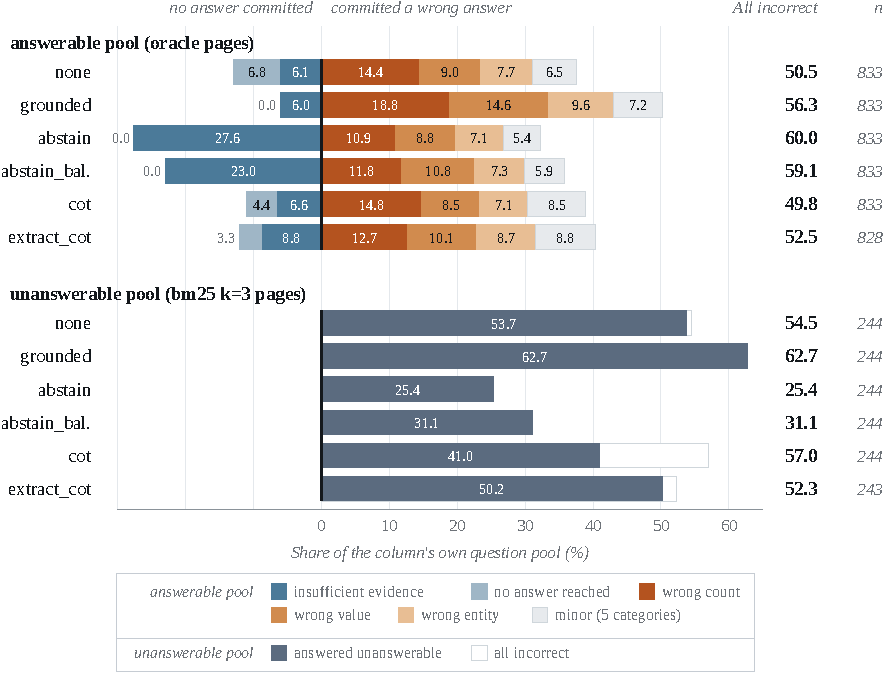
\includegraphics[width=0.8\columnwidth]{empirical/analysis/error_profile.pdf}
  \caption[Error profile by prompt mode]{Error profile by prompt mode on answerable and unanswerable questions. Answerable errors are decomposed by failure type, while the unanswerable pool reports unsupported answers. Grounding primarily shifts non-commitment into explicit errors, while chain-of-thought leaves answerable accuracy largely unchanged and increases unsupported answering on unanswerable questions.}
  \label{fig:error_profile}
\end{figure}

\paragraph{Grounding Encourages Commitment Without Improving Reliability.} The grounded prompt removes one visible failure mode, but largely by shifting errors rather than preventing them. On the answerable pool, \emph{no answer reached} falls from 6.8\% to 0.0\%, yet wrong-count, wrong-value, and wrong-entity errors all increase. The same tendency appears on the unanswerable pool, where the rate of answered-unanswerable questions rises from 54.5\% to 62.7\%. Grounding therefore appears to make the model more willing to commit to an answer without improving whether that answer is supported or correct.

\paragraph{Chain-of-Thought Does Not Improve Calibration.} Chain-of-thought prompting produces almost no change in overall performance on answerable questions, with the total incorrect rate moving from 50.5\% to 49.8\%. More surprisingly, it performs worse on the unanswerable pool, where 57.0\% of questions are answered despite the evidence being insufficient. This runs counter to the expectation that explicit reasoning should help the model recognise when the available evidence cannot support an answer. Instead, longer reasoning may encourage the model to construct or rationalise an answer from incomplete context rather than identify the missing evidence. Reasoning longer is therefore not equivalent to reasoning about evidential sufficiency.

\subsection{Error Patterns by Evidence and Integration}
\label{sec:error_evidence_integration}

\begin{figure}[ht]
  \centering
  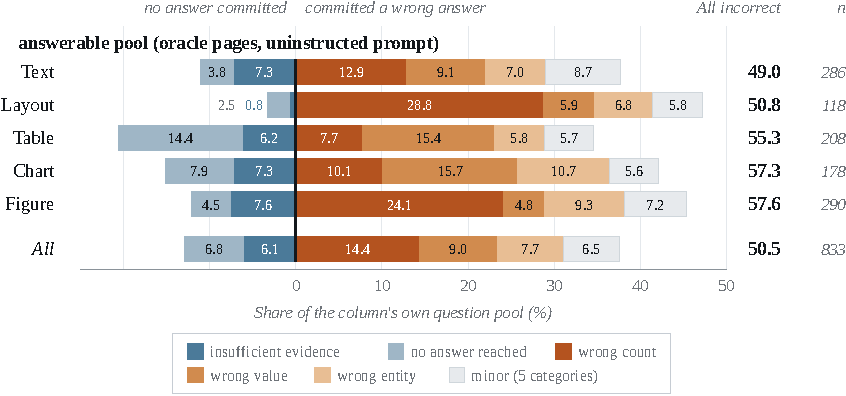
\includegraphics[width=0.8\columnwidth]{empirical/analysis/error_sources.pdf}
  \caption[Error profile by evidence source]{Error profile by evidence source on the answerable pool with oracle pages and no prompt instruction. Different evidence types produce distinct failure patterns: layout and figure questions are dominated by wrong-count errors, while tables and charts more often produce wrong-value errors.}
  \label{fig:error_sources}
\end{figure}

\paragraph{Error Type Depends on the Evidence Being Interpreted.} The evidence-source breakdown shows that different modalities do not simply vary in overall difficulty, but fail in different ways. Layout and figure questions are dominated by wrong-count errors, reaching 28.8\% and 24.1\%, which is consistent with difficulty identifying or enumerating visually distributed elements. Tables and charts instead show larger wrong-value errors at 15.4\% and 15.7\%, suggesting that the relevant structure is often located but the wrong numeric value is extracted or used. Tables also show a comparatively high no-answer-reached rate of 14.4\%, indicating that structured evidence can cause the reasoning process to fail before a final answer is committed. Evidence source therefore affects not only whether the model fails, but the form that failure takes.

\begin{figure}[ht]
  \centering
  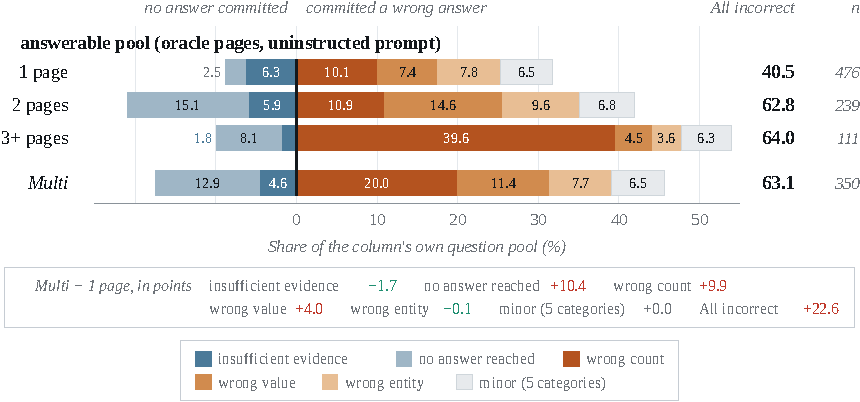
\includegraphics[width=0.8\columnwidth]{empirical/analysis/error_integration.pdf}
  \caption[Error profile by evidence-page count]{Error profile by evidence-page count on the answerable pool with oracle pages and no prompt instruction. Moving from single-page to multi-page questions sharply increases non-commitment, wrong-count, and wrong-value errors, while insufficient-evidence errors do not increase.}
  \label{fig:error_integration}
\end{figure}

\paragraph{Cross-Page Integration Amplifies Reasoning Errors.} Moving from one page to multiple pages produces a clear shift in the error profile. Relative to single-page questions, the pooled multi-page set shows a 10.4-point increase in no-answer-reached errors, a 9.9-point increase in wrong-count errors, and a 4.0-point increase in wrong-value errors. By contrast, insufficient-evidence errors decrease slightly. Since every oracle page is supplied, these failures are not caused by missing evidence, but by difficulty combining and operating over evidence that is already present. The largest change also occurs when moving from one page to two pages, with total incorrect rising from 40.5\% to 62.8\%, while 3+ pages reach 64.0\%. This suggests that crossing the page boundary itself introduces much of the reasoning burden, rather than error increasing proportionally with each additional page.

\section{Practical Discussion}
\label{sec:practical_discussion}

The preceding experiments isolate where MP-VRDU systems fail. We now consider what those findings imply for system design and deployment. Rather than treating representation, retrieval, and reasoning independently, the results suggest that compute should be allocated across the pipeline according to where information is most likely to be lost and where additional capacity can still recover it.

\subsection{Representation Cost and Fidelity}
\label{sec:discussion_representation}

% GENERATED by tables/scripts/ -- do not edit by hand, re-run the script.
% Numbers read from results/tables/analysis/*.csv (cost) and mmlongbench/*.csv (OOM).
% deployment_rungs (results.errcat.jsonl), oom_frontier
% Teal deepens with accuracy on Ladder.tex's fixed [14,74] scale, so a cell here reads
% against a cell there. Warm wash on input tokens and on the OOM rate: both are costs.
\definecolor{accteal}{HTML}{1BAF7A}
\definecolor{recwarm}{HTML}{D95926}

\begin{table}[ht]
\centering
\small
\setlength{\tabcolsep}{5pt}
\renewcommand{\arraystretch}{1.12}
\begin{tabular}{@{}l r rrr r rr r@{}}
\toprule
 & & \multicolumn{3}{c}{\textbf{Input tokens}} & & \multicolumn{2}{c}{\textbf{Output}} & \\
\cmidrule(lr){3-5}\cmidrule(lr){7-8}
\textbf{Rung} & \textbf{Acc.} & \textbf{text} & \textbf{visual} & \textbf{total} & \textbf{prefill s} & \textbf{tok} & \textbf{decode s} & \textbf{OOM \%} \\
\midrule
\textbf{T} & \cellcolor{accteal!15}29.0 & 932 & 0 & \cellcolor{recwarm!9}932 & 1.4 & 115 & 5.7 & \cellcolor{recwarm!2}1.2 \\
\textbf{TL} & \cellcolor{accteal!22}35.7 & 1632 & 0 & \cellcolor{recwarm!16}1632 & 1.8 & 133 & 6.6 & \cellcolor{recwarm!9}6.7 \\
\textbf{TV} & \cellcolor{accteal!36}50.1 & 929 & 3404 & \cellcolor{recwarm!43}4333 & -- & 140 & -- & -- \\
\textbf{TLV} & \cellcolor{accteal!36}49.5 & 1632 & 3427 & \cellcolor{recwarm!51}5058 & 26.3 & 136 & 6.7 & \cellcolor{recwarm!15}11.2 \\
\textbf{V} & \cellcolor{accteal!29}42.6 & 38 & 3427 & \cellcolor{recwarm!35}3464 & 29.0 & 139 & 7.1 & \cellcolor{recwarm!1}0.8 \\
\bottomrule
\end{tabular}
\caption{Cost of each representation rung. Accuracy and token counts are means over the answerable pool under the error-taxonomy judge; the two latency columns and the OOM rate are measured separately on 2$\times$16\,GB V100s, the hardware the study deploys on. Adding the page image is what costs: prefill rises roughly fifteen-fold from \textbf{TL} to \textbf{TLV} while decode barely moves.}
\label{tab:deployment_rungs}
\end{table}

% {\footnotesize\raggedright
% Uninstructed prompt, oracle pages, answerable pool, judged under the error-taxonomy
% rubric. Accuracy is the same judge and the same pool as Table~\ref{tab:ladder_source} and
% shares its teal scale, so a cell here reads against a cell there; it is NOT interchangeable
% with a level from a table scored by the main report's judge.
% \textbf{Input and output cost are set by different things and must be read apart.} Input
% tokens and prefill time are fixed by the representation: TL adds parser markdown to T, V
% replaces text with about 3,400 visual tokens, and TLV pays for both. Output tokens and decode
% time are set by the prompt and the decode budget, so they barely move across rungs; a rung
% that appears to decode more is one whose longer input drew a longer answer. The two halves do
% not sum to end-to-end latency, which also carries scheduling and detokenisation.
% \textbf{The three right-hand columns are measured on different rows from the accuracy.}
% Latency and the OOM rate both read the preserved pre-recovery V100 snapshots, because this
% pool's failed cells were re-run on an H100: the live rows carry that machine's timings, where
% the same cells prefill in 0.06--0.18\,s and \textbf{TL}$\rightarrow$\textbf{TLV} rises
% 1.8-fold rather than 13.6-fold, which prices the table on hardware the study does not deploy
% on. Latency is therefore a mean over the matched cells every ladder config ran ($n=831/761/717/834$
% by rung), which excludes the cells that OOMed and so prices a lighter input than the token
% columns show: \textbf{TLV} averages 3,501 tokens over those cells against 5,058 over the
% full pool. The OOM rate is the same snapshot pooled over its page-count buckets at medium
% resolution. \textbf{TV} never ran on a V100, so it carries no latency and no rate; its cost
% sits in the token columns, which are machine-independent. Latency is wall clock and a scale
% rather than an absolute. Table~\ref{tab:reasoner_cost_all} gives the same two columns for
% every reasoner configuration, grouped by measuring machine.
% \textbf{TV is the rung that pays for itself, and under this judge it beats TLV outright.}
% It scores 50.1 against 49.5 on 725 fewer input tokens, so \textbf{TLV} is dominated: it costs
% more and returns less. The parser's markdown does not merely earn little once the page image
% is present, it is a net loss. Read the two accuracies as close rather than as a ranking: TV is
% measured over all 847 cells and the other rungs over the 833 the sweep judged, and the
% difference is well inside either interval.\par}

\paragraph{Representation Should Match the Deployment Constraint.} Table~\ref{tab:deployment_rungs} shows that the main practical cost of richer representations comes from visual input, which increases context size and memory pressure far more than text-only encoding. This matters because deployment budgets are shared across page count, batch size, latency, and accelerator memory. The representation findings in Table~\ref{tab:ladder_source} show that vision is essential for some evidence sources, while Table~\ref{tab:resolution_sweep} shows that visual fidelity itself also carries a cost. A deployed system should therefore treat representation as a resource-allocation decision. Visual input is justified when the workload contains evidence that text cannot preserve, but using it indiscriminately reduces the number of pages or queries that can be processed within the same hardware budget.

\paragraph{The Best Representation Is Not Always the Best Deployment Choice.} In capability terms, a sufficiently strong reasoner should benefit from retaining the richest available evidence, but real-world systems rarely operate without compute constraints. The modality results in Table~\ref{tab:ladder_source} and parser results in Figure~\ref{fig:parser} suggest that the appropriate representation depends on the expected document and question distribution. For predominantly textual, born-digital workloads such as academic papers, embedded or parsed text may preserve most of the required evidence at substantially lower cost. Scanned, figure-heavy, chart-heavy, or layout-sensitive workloads are more likely to justify visual input. Mixed deployments can instead escalate selectively, using a cheaper text representation by default and invoking vision only when the document or question requires it. The practical objective is therefore not to maximise representation richness, but to use the cheapest representation that preserves the evidence required by the target workload.

\subsection{Retrieval Quality and Efficiency}
\label{sec:discussion_retrieval}

\begin{figure}[ht]
  \centering
  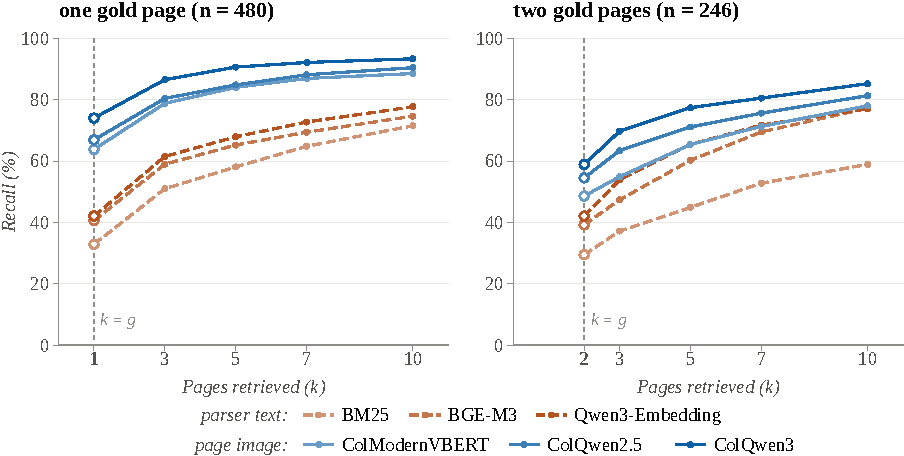
\includegraphics[width=0.9\columnwidth]{empirical/discussion/retrieval.pdf}
  \caption[Retrieval recall by depth and gold-page count]{Retrieval recall by depth and gold-page count on MMLongBench-Doc. Recall increases consistently with retrieval depth, while questions requiring two gold pages remain harder to cover than single-page questions.}
  \label{fig:retrieval}
\end{figure}

\paragraph{Retrieval Depth Should Favour Recall.} As Figure~\ref{fig:retrieval} shows, recall rises steadily with retrieval depth across all six retrievers, and the two-gold-page pool remains harder to cover than the one-gold-page pool at the same \(k\). In deployment, the operating point should therefore be chosen around an acceptable coverage target rather than precision in isolation. A larger \(k\) may be justified for questions likely to depend on several pages, while simpler or highly localised tasks can stop earlier. Retrieval itself is comparatively inexpensive once the index is built, so the main practical cost of increasing \(k\) is the additional reasoner context and generation latency incurred when more pages are subsequently processed.

\begin{figure}[ht]
  \centering
  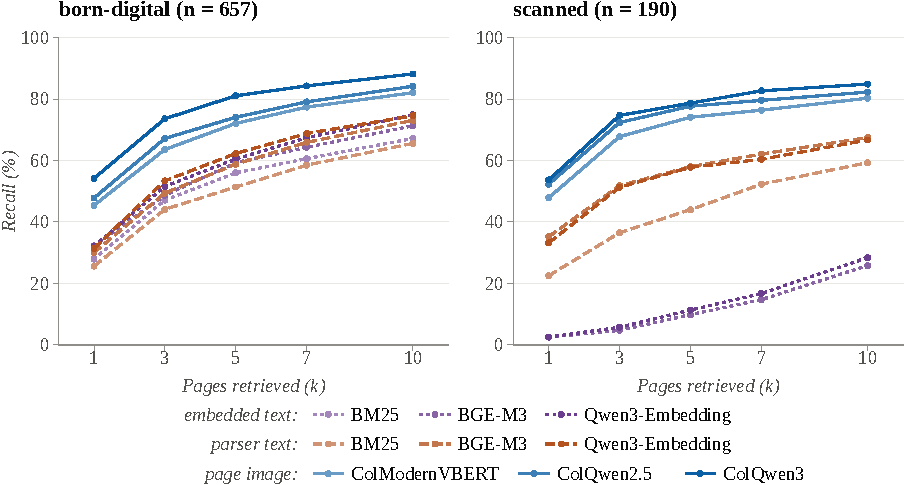
\includegraphics[width=0.9\columnwidth]{empirical/discussion/retrieval_scan.pdf}
  \caption[Retrieval recall by document type and retrieval representation]{Retrieval recall by document type and retrieval representation on MMLongBench-Doc. Parser-based text retrieval substantially improves robustness on scanned documents, while visual retrievers remain strongest and most consistent across both document types.}
  \label{fig:retrieval_scan}
\end{figure}

\paragraph{Retrieval Representation Trades Cost for Robustness.} Figure~\ref{fig:retrieval_scan} shows that retrieval representation affects robustness as well as preprocessing cost. Embedded-text retrieval is inexpensive because it can use the existing PDF text layer, but it degrades sharply on scanned documents. Parser-text retrieval adds conversion overhead while recovering much of this lost performance, and visual retrieval requires page rendering and visual embedding but remains the strongest and most consistent across document types. The resulting trade-off is therefore not simply text versus vision. Once the corresponding indexes are precomputed, query-time retrieval remains small relative to multimodal generation, making representation choice primarily a balance between document-preparation cost and retrieval robustness.


\subsection{Reasoner Capability and Deployment Trade-offs}
\label{sec:discussion_reasoner}

% GENERATED by tables/scripts/ -- do not edit by hand, re-run the script.
% Numbers read from results/tables/mmlongbench/*.csv.
% reasoner_unified, weight_footprint
% Teal deepens with accuracy on Ladder.tex's fixed [14,74] scale, so a cell here reads
% against a cell there. GB carries its own warm scale over [4,25]: a footprint is a
% cost, not an accuracy. Empty rows are models declared but not yet run.
\definecolor{accteal}{HTML}{1BAF7A}
\definecolor{recwarm}{HTML}{D95926}

\begin{table}[ht]
\centering
\small
\setlength{\tabcolsep}{4pt}
\begin{tabular}{lrrrrr}
\toprule
\textbf{Model / config} & \textbf{T} & \textbf{TL} & \textbf{TLV} & \textbf{V} & \textbf{GB} \\
\midrule
\multicolumn{6}{l}{\emph{Scale (Qwen3-VL, bf16)}} \\
\quad 2B & \cellcolor{accteal!11}24.7 & \cellcolor{accteal!18}31.9 & \cellcolor{accteal!24}38.3 & \cellcolor{accteal!18}31.9 & \cellcolor{recwarm!1}4.3 \\
\quad 4B & \cellcolor{accteal!18}32.3 & \cellcolor{accteal!25}38.6 & \cellcolor{accteal!36}50.4 & \cellcolor{accteal!28}42.4 & \cellcolor{recwarm!13}8.9 \\
\quad 8B & \cellcolor{accteal!18}31.9 & \cellcolor{accteal!24}38.4 & \cellcolor{accteal!38}52.4 & \cellcolor{accteal!32}45.5 & \cellcolor{recwarm!35}17.5 \\
\quad 32B & \cellcolor{accteal!22}35.5 & \cellcolor{accteal!30}43.9 & \cellcolor{accteal!46}59.6 & \cellcolor{accteal!43}56.7 & \cellcolor{recwarm!55}66.7 \\
\cmidrule(lr){1-6}
\multicolumn{6}{l}{\emph{Precision (Qwen3-VL-8B)}} \\
\quad 16-bit & \cellcolor{accteal!18}31.9 & \cellcolor{accteal!24}38.4 & \cellcolor{accteal!38}52.4 & \cellcolor{accteal!32}45.5 & \cellcolor{recwarm!35}17.5 \\
\quad 8-bit & \cellcolor{accteal!18}32.5 & \cellcolor{accteal!24}37.9 & \cellcolor{accteal!40}53.6 & \cellcolor{accteal!32}45.7 & \cellcolor{recwarm!16}10.3$^{\sim}$ \\
\quad 4-bit & \cellcolor{accteal!18}31.8 & \cellcolor{accteal!25}39.4 & \cellcolor{accteal!38}51.8 & \cellcolor{accteal!32}45.5 & \cellcolor{recwarm!7}6.8$^{\sim}$ \\
\cmidrule(lr){1-6}
\multicolumn{6}{l}{\emph{Matched budget ($\sim$17--20\,GB)}} \\
\quad 8B, 16-bit & \cellcolor{accteal!18}31.9 & \cellcolor{accteal!24}38.4 & \cellcolor{accteal!38}52.4 & \cellcolor{accteal!32}45.5 & \cellcolor{recwarm!35}17.5 \\
\quad 32B, 4-bit & \cellcolor{accteal!23}37.0 & \cellcolor{accteal!28}42.1 & \cellcolor{accteal!45}59.1 & \cellcolor{accteal!38}52.3 & \cellcolor{recwarm!42}20.0$^{\sim}$ \\
\cmidrule(lr){1-6}
\multicolumn{6}{l}{\emph{Family (8B class, bf16)}} \\
\quad Qwen3-VL-8B & \cellcolor{accteal!18}31.9 & \cellcolor{accteal!24}38.4 & \cellcolor{accteal!38}52.4 & \cellcolor{accteal!32}45.5 & \cellcolor{recwarm!35}17.5 \\
\quad InternVL3-8B & \cellcolor{accteal!5}19.3 & \cellcolor{accteal!11}25.3 & \cellcolor{accteal!19}32.6 & \cellcolor{accteal!10}24.1 & \cellcolor{recwarm!31}15.9 \\
\quad GLM-4.6V-Flash (9B dense) & \cellcolor{accteal!12}25.8 & \cellcolor{accteal!20}33.5 & \cellcolor{accteal!30}44.1 & \cellcolor{accteal!17}31.0 & \cellcolor{recwarm!43}20.6 \\
\quad MiniCPM-V-4.5 (8B) & \cellcolor{accteal!17}30.8 & \cellcolor{accteal!24}37.9 & \cellcolor{accteal!48}61.9 & \cellcolor{accteal!40}53.8 & \cellcolor{recwarm!35}17.4 \\
\quad Llama-3.2-11B-Vision & \cellcolor{accteal!12}26.5 & \cellcolor{accteal!20}34.3 & \cellcolor{accteal!19}33.3 & \cellcolor{accteal!11}25.3 & \cellcolor{recwarm!45}21.3 \\
\cmidrule(lr){1-6}
\multicolumn{6}{l}{\emph{Scale (Gemma-3, bf16)}} \\
\quad 4B & \cellcolor{accteal!8}22.1 & \cellcolor{accteal!16}30.4 & \cellcolor{accteal!26}39.9 & \cellcolor{accteal!20}33.8 & \cellcolor{recwarm!12}8.6 \\
\quad 12B & \cellcolor{accteal!16}30.4 & \cellcolor{accteal!24}37.5 & \cellcolor{accteal!37}50.9 & \cellcolor{accteal!29}42.6 & \cellcolor{recwarm!53}24.4 \\
\quad 27B & -- & -- & -- & -- & \cellcolor{recwarm!55}54.9 \\
\cmidrule(lr){1-6}
\multicolumn{6}{l}{\emph{Sparse (mixture of experts)}} \\
\quad Qwen3-30B-A3B-Instruct & -- & -- & -- & -- & -- \\
\cmidrule(lr){1-6}
\multicolumn{6}{l}{\emph{Reasoning variant (Qwen3-VL-8B, TLV only)}} \\
\quad Instruct & \cellcolor{accteal!18}31.9 & \cellcolor{accteal!24}38.4 & \cellcolor{accteal!38}52.4 & \cellcolor{accteal!32}45.5 & \cellcolor{recwarm!35}17.5 \\
\quad Thinking & -- & -- & \cellcolor{accteal!48}62.2 & -- & \cellcolor{recwarm!35}17.5 \\
\bottomrule
\end{tabular}
\caption{Reasoner accuracy across scale, precision, matched budget and family. Accuracy (\%) on oracle pages over the full answerable pool; GB is the model weight footprint, not peak VRAM.}
\label{tab:reasoner}
\end{table}

% {\footnotesize\raggedright
% Accuracy (\%) on oracle pages at medium resolution, uninstructed prompt, full answerable
% pool ($n=847$); per-cell $n$ is omitted for space and runs 640--847, thinnest at TLV where
% OOM attrition is largest. Teal shares Table~\ref{tab:ladder_source}'s scale, so a cell here
% reads against a cell there. \textbf{GB} is the model weight footprint, carrying its own warm
% scale because a footprint is a cost rather than an accuracy; $^{\sim}$ marks a footprint
% derived from the 16-bit weights rather than measured. Peak VRAM was device-0 only and is not
% reported. \textbf{Empty rows are models declared in the methodology that have not been run.}
% \textbf{Scale buys the most on the visual rungs} and quantization is nearly free: 4-bit
% costs the 8B 0.6 points at TLV for 61\% of the weights. At a matched memory budget the
% quantized 32B beats the 16-bit 8B at every rung, which is the practical reading of the
% table: given a fixed card, a larger model at lower precision is the better buy. \textbf{Family
% choice costs more than either}, and in both directions: at essentially the same footprint
% InternVL3-8B loses 19.8 points to Qwen3-VL-8B at TLV while MiniCPM-V-8B gains 9.5, a spread
% wider than four times the scale step from 2B to 32B. The family is the first decision, not
% the last. MiniCPM-V's thinner $n$ at TLV (640) is OOM attrition, so read that cell as a
% surviving-question rate rather than a like-for-like win. \\textbf{Llama-3.2-11B-Vision is the
% one family that loses accuracy when the pages are added}: it peaks at TL (34.3) and drops to
% 33.3 at TLV and 25.3 at V, so for it the ladder inverts and the parser text is the better
% input. Every other family gains on the visual rungs.
% \textbf{The Thinking checkpoint ran at TLV only} and gains 9.8 points there over the
% Instruct model it forks from, the largest single move in the table; its value is in the
% hop split rather than the level, since it nearly closes the multi-page deficit
% ($-$9.1 against $-$19.9). \textbf{GLM-4.6V} is the 107B mixture-of-experts member of the
% GLM line, a different architecture from the 9B dense Flash variant above rather than a
% size option of it, and has not been run.\par}

\paragraph{Reasoner Choice Is a Capability--Efficiency Trade-off.} The choice of reasoner reflects the broader capability--efficiency trade-off that underlies modern language and multimodal model deployment. Increasing model scale can improve task capability, but parameter count alone is an imperfect predictor of performance. As Table~\ref{tab:reasoner} shows, similarly sized model families differ substantially on MP-VRDU, while scaling within a family generally improves accuracy at considerable memory and compute cost. This makes model selection a joint decision over architecture, scale, token efficiency, and the target workload rather than a simple preference for the largest available checkpoint. The cost is particularly relevant for MP-VRDU because each query may already contain thousands of textual and visual tokens. In practice, organisations should therefore benchmark candidate model families on their own document distribution and choose the model that provides sufficient capability within the available latency, memory, and throughput budget.

\paragraph{Quantisation Can Preserve Capacity Under a Fixed Memory Budget.} Quantisation changes this trade-off without substantially reducing accuracy in our experiments. Table~\ref{tab:reasoner} shows that reducing Qwen3-VL-8B from 16-bit to 8- or 4-bit precision changes accuracy only slightly across the tested representations while reducing its weight footprint from 17.5\,GB to approximately 10.3 and 6.8\,GB. This contrasts with studies reporting larger degradation under low-bit quantisation on long-context and reasoning-intensive tasks~\cite{mekala2025quantization,li2025quantization,marchisio2024quantization}. One possible explanation is that many document QA instances require comparatively constrained operations over already supplied evidence, such as recovering an entity, count, or value, making them less sensitive to small weight perturbations than extended reasoning or generation. Quantisation also does not increase latency in our measurements and produces a small improvement, consistent with prior work showing that well-supported low-precision inference can improve deployment efficiency~\citep{kurtic2025quantization}. More importantly, the 4-bit 32B model outperforms the 16-bit 8B model across all four representation rungs at a similar weight budget. For fixed-memory deployment, reducing numerical precision may therefore be preferable to reducing model scale, although this result should not be interpreted as evidence that low-precision inference is generally lossless.


\section{Conclusion}
\label{sec:emp-conc}

This chapter examined MP-VRDU failure through controlled attribution across representation, selection, and reasoning. The results show that vision is necessary but remains complementary to text, that missing required evidence is substantially more damaging than moderate distractor exposure, and that cross-page integration remains difficult even when all required evidence is supplied. The analysis further shows that prompt interventions can shift error behaviour without necessarily improving underlying reasoning or calibration. Together, these findings show that MP-VRDU failure is distributed across the evidence pipeline and that end-to-end accuracy alone is insufficient to identify the mechanism responsible.